\documentclass[12pt]{article}
\usepackage{fullpage}
\usepackage{graphicx, rotating, booktabs} 
\usepackage{times} 
\usepackage{fbb} 
\usepackage{natbib} 
\usepackage{indentfirst} 
\usepackage{setspace}
\usepackage{grffile} 
\usepackage{hyperref}
\usepackage{tikz-cd}
 \usetikzlibrary{cd}
\usepackage[export]{adjustbox}
\usepackage[most]{tcolorbox}
\usepackage{verbatimbox}
\usepackage{lscape}
\usepackage{afterpage}
\usepackage{amsmath}
\usepackage[labelfont={bf},textfont=it,labelsep=period]{caption}
 \usepackage{multirow} 
\setcitestyle{aysep{}}
\usepackage{dcolumn}

\hypersetup{
  colorlinks = true,
  urlcolor = blue,
  linkcolor = black,
  citecolor = black,
  pdfauthor = {Joshua Alley},
  pdfkeywords = {},
  pdftitle = {},
  pdfsubject = {},
  pdfpagemode = UseNone,
%  pdffitwindow = true
%  pdfcenterwindow = true
}



\singlespace
\title{\textbf{Alliances, Arms Exports and Electoral Trade Cycles}}
\author{Joshua Alley \\
Postdoctoral Research Associate \\
University of Virginia\thanks{Thanks to Brian Blankenship, Jonathan Caverley, Jonathan Chu, Lauren Peritz, Erik Lin-Greenberg, Zachary Markovitch and participants in the Boston University Political Economy of Security Online Workshop Series and 2022 Meeting of the International Studies Association for helpful comments.} \\
jkalley@virginia.edu
}

 
\date{\today}

\bibliographystyle{apsr}

\usepackage{sectsty}
\sectionfont{\Large}
\subsectionfont{\noindent\large\textit}
\subsubsectionfont{\normalsize}

\makeatletter
\renewcommand\tiny{\@setfontsize\tiny{9}{10}}
\makeatother


\begin{document}

\maketitle 

\begin{abstract} 
Political budget cycles in the United States increase international trade, especially arms exports to allies. 
When U.S. allies purchase weapons and accept arms transfers, they provide an outlet for outputs from efforts to use defense contracting to stimulate economic growth in key electoral areas.
Presidents and senators employ defense contracts because they have more control over this policy instrument than aggregate economic tools.
Alliance proteges' positive economic and security statecraft thus helps U.S. leaders manipulate the economy during leadership competitions.  
I examine these claims with three analyses of trade, arms transfers and defense contracting in the United States. 
First, I show that U.S. trade cycles track elections, with substantial increases in overall trade and exports to allies near elections.
I then detail corresponding electoral cycles in arms exports from the United States to allies. 
Finally, I provide initial evidence of increased defense contract awards around elections.
The results suggest that security and economic ties provide alliance patron leaders with avenues for electoral gain. 
\end{abstract} 


\newpage 
\doublespace 


\section{Introduction}


% start with a good story of increased trade near elections: compare ally/not 
% Matching for case selection produces: 1996 Denmark and Sweden
U.S. trade with Denmark and Sweden spiked in 1996, as Bill Clinton ran for re-election.
Exports to and imports from both Nordic countries rose, but Denmark received more U.S. exports.
While these countries occupied similar regions and shared similar trade relations with the United States, Denmark received more exports because U.S. arms exports to this NATO member also rose.


% give another example: Turkey and Egypt 1984
Two Middle Eastern states experienced similar trade changes in 1984 when Ronald Reagan stood for a second term.
U.S. trade with Turkey and Egypt grew, but exports to Turkey increased more than exports to Egypt. 
As in the Denmark and Sweden case, Turkey had a formal U.S. security guarantee and Egypt did not, so Turkey received greater U.S. arms transfers and thus higher exports. 


% example- PBC consequences vary w/ security coop
These cases reflect a more general pattern, where presidential elections in the United States expand international trade, especially arms exports to allies.
This paper unpacks the role of alliances and arms transfers in electoral trade cycles between the United States and other countries. 
I argue that U.S. allies receive more exports due to arms transfers from defense contracting cycles. 


% arms exports logic
Security cooperation facilitates electoral cycles in arms exports. 
U.S. leaders produce additional arms by using defense contracting to create domestic political business cycles \citep{Tufte1978, Mintz1988, Mayer1995, DerouenHeo2000, Becker2021}.
Alliance proteges provide a key market for exports from defense contracting cycles.
Allies receive more arms from their patrons near elections because they control import decisions and receive security benefits. 
These arms export cycles reinforce cooperative relationships between U.S. leaders and alliance proteges.


Along with tracking defense contracting cycles, I examine the arms exports argument by showing that security factors do not modify electoral electoral trade cycles in imports.
In addition to defense contracting, elected leaders often use fiscal and monetary policy \citep{Nordhaus1975, Tufte1978, Rogoff1987, ClarkHallerberg2000} to boost economic growth around elections. 
Economic expansion from political business cycles in large states pulls in more imports.
Because foreign firms respond to increased domestic demand regardless of security relations, import cycles near elections serve as an important placebo check on the exports results.


% Findings
I examine how U.S. allies facilitate electoral export cycles in three ways. 
First, I show that U.S. exports to allies increase more than exports to non-allies near presidential elections. 
I then demonstrate corresponding cycles in arms transfers, where arms exports to allies rise as elections approach, and provide descriptive evidence of underlying defense contracting cycles.
Finally, I use section 655 reports to link international arms transfer agreements and contract awards by sector in an analysis from YEAR to YEAR.


% focus on the U.S.
The argument and analysis focus on the United States because it has the largest economy, substantial alliance ties, and prior evidence of defense contracting cycles. 
Electoral trade and arms transfer cycles will likely be weaker in other countries with smaller economies and defense industries. 
Still, the pivotal economic and security roles of the United States make understanding the economic and security consequences of U.S. political budget cycles worthwhile.
Furthermore, similar trade cycles may occur in other states with different policy cycles. 


% economic and seucrity ties 
The argument and findings address three salient issues in international relations theory and practice. 
First, they detail the international consequences of political budget cycles. 
Domestic political business cycles in large countries like the United States reshape international economic exchanges and have knock-on effects in other countries.
International economic expansions and related domestic growth make early elections in parliamentary democracies more likely \citep{Kayser2006} and increase vote shares for parties supporting higher taxes and spending \citep{Kayser2009}, to give two examples.


Second, I speak to debates about how economic and security ties interact \citep{Mastanduno2009, Poast2019}. 
Scholars dispute whether economic linkages drive security ties \citep{BiglaiserDeRouen2007, Fordham2010, Kimball2010}, security concerns encourage economic linkages \citep{Gowa1995, Li2003, LongLeeds2006, GowaMansfield2004}, or both \citep{BiglaiserDeRouen2009, KinneBunte2018}. 
My findings suggest that this relationship varies with electoral cycles, countries and sectors.


Another related body of research on economic bargaining in asymmetric alliances like those between the United States and its partners falls into two camps. 
One argues that alliance patrons have limited economic leverage because they prioritize geopolitical aims \citep{Drezner2013, WolfordKim2017}.
Another perspective claims that alliance leaders have substantial economic influence \citep{Norrlof2010, Brooksetal2013} and threats to reduce security commitment encourage economic concessions \citep[pg. 122]{Oatley2015}.
Rather than analyze coercive economic demands, my argument covers how positive economic statecraft helps U.S. leaders advance their electoral interests.


% coercion
Finally, this paper provides new insight into economic statecraft. 
Most economic statecraft scholarship studies economic sanctions (e.g. \cite{Marinov2005, Allen2008, Escriba-FolchWright2010}).
But as \citet{Baldwin2020} notes, economic statecraft includes positive inducements and negative sanctions. 
This paper examines positive economic statecraft--- how alliance proteges use political economy decisions to indirectly facilitate patron leaders' political budget cycles.
As a result, it connects with prior work on issue linkage in alliance management, including studies of alliance formation \citep{Poast2012} and credibility \citep{Davis2008, Poast2013}. 


These claims complement prior findings that foreign states use economic policies to manipulate electoral competition. 
\citet{KimMargalit2021} find that Chinese tariffs reduced Republican vote share in the 2018 midterm elections by targeting industries in competitive districts.
In the same way, \citet{ChyzhUrbatsch2021} find that Chinese soy tariffs hurt Republican congressional candidates in soy-producing areas. 
My argument inverts this logic by examining how security allies accommodate electoral budget cycles and thereby help incumbents win office. 


% policy 
My finding that allies assist political budget cycles through arms exports has important implications for alliance durability. 
Leaders who anticipate benefiting from allied trade cycles will be more likely to demonstrate and uphold alliance commitment. 
Electoral trade cycles are therefore a potential component of grand bargains between alliance patrons and their proteges. 


% need an outline 
The paper proceeds as follows. 
To start, I outline an argument detailing the international economic consequences of political business cycles in the United States, the role of defense contracting in those cycles, and the consequences for international trade as well as exports to allies.
I then test the process in three steps. 
First, I show that U.S. exports to allies increase more as elections approach, relative to states without a defense pact. 
I then demonstrate that arms exports from the United States to allies mirror the electoral export cycle.
Third, I establish the political business cycle roots of arms exports with evidence of defense contracting cycles.
The last section discusses the results and offers concluding thoughts.


\section{Argument}


This argument explains how alliances reshape the international economic consequences of domestic political business cycles. 
First, I detail how political budget cycles expand overall trade.
I then discuss how presidential control makes defense contracting an attractive policy tool for manipulating economic conditions around elections. 
After that, allies provide an market for outputs from electoral cycles in defense contracting. 
The net outcome is general electoral trade cycles with greater exports to allies through arms transfers. 


Electoral considerations impact economic policy \citep{Nordhaus1975}.\footnote{See \citet{Dubois2016} for a review of this vast literature.} 
Leaders undertake political budget cycles by using fiscal and monetary policy to increase economic growth near elections and retain power for themselves or their party \citep{Tufte1978, Rogoff1987}. 
The composition and magnitude of these cycles varies. 
For example, strong central bank interdependence and fixed exchange rates make fiscal cycles more likely \citep{ClarkHallerberg2000}. 
Even some independent central banks exhibit modest cyclical behavior, however \citep[pg. 247]{Dubois2016}


% Political Business cyles
By creating domestic business cycles with higher growth near elections, political budget cycles have international economic consequences.
Fiscal and monetary policy shifts impact currency prices and economic growth, which then alters trade and financial ties. 
The larger the economy, the greater the international economic consequences of political business cycles.
Economic interdependence leads to correlated economic growth across countries \citep{ArtisZhang1999, Kayser2006} and increases the global economic influence of large economies. 
\citet{Ito1991} finds that U.S. elections increase economic growth in Japan, while \citet{ThompsonZuk1983} uncover some evidence of similar cycles in advanced industrial economies.
\citet{FoersterSchmitz1997} argue that U.S. electoral cycles impact international stock returns.


% increased domestic consumption- 
There is less empirical evidence of electoral trade cycles, but the theory is straightforward.
For example, monetary expansion has price and income effects--- price effects of currency devaluation make exports more competitive, while increased incomes stimulate import consumption \citep{Sumner2021}.
Economic growth from political budget cycles also increases domestic consumption and demand for imported goods. 
Electoral cycles in imports follow, as consumption follows economic expansions and contractions from political budget cycles.  
While all economies with political budget cycles should pull in additional trade near elections, these effects will be more pronounced in large economies. 


There are clear electoral cycles in U.S. exports, imports and total trade from 1951 to 2019. 
\autoref{fig:us-trade-cycles} presents the distribution of annual changes in logged exports, imports and overall trade as presidential elections approach.
Box plots summarize the distribution of U.S. trade with all states in the years after to years of presidential elections. 
The dark line in each box plot marks the median value. 


\begin{figure}
\centering
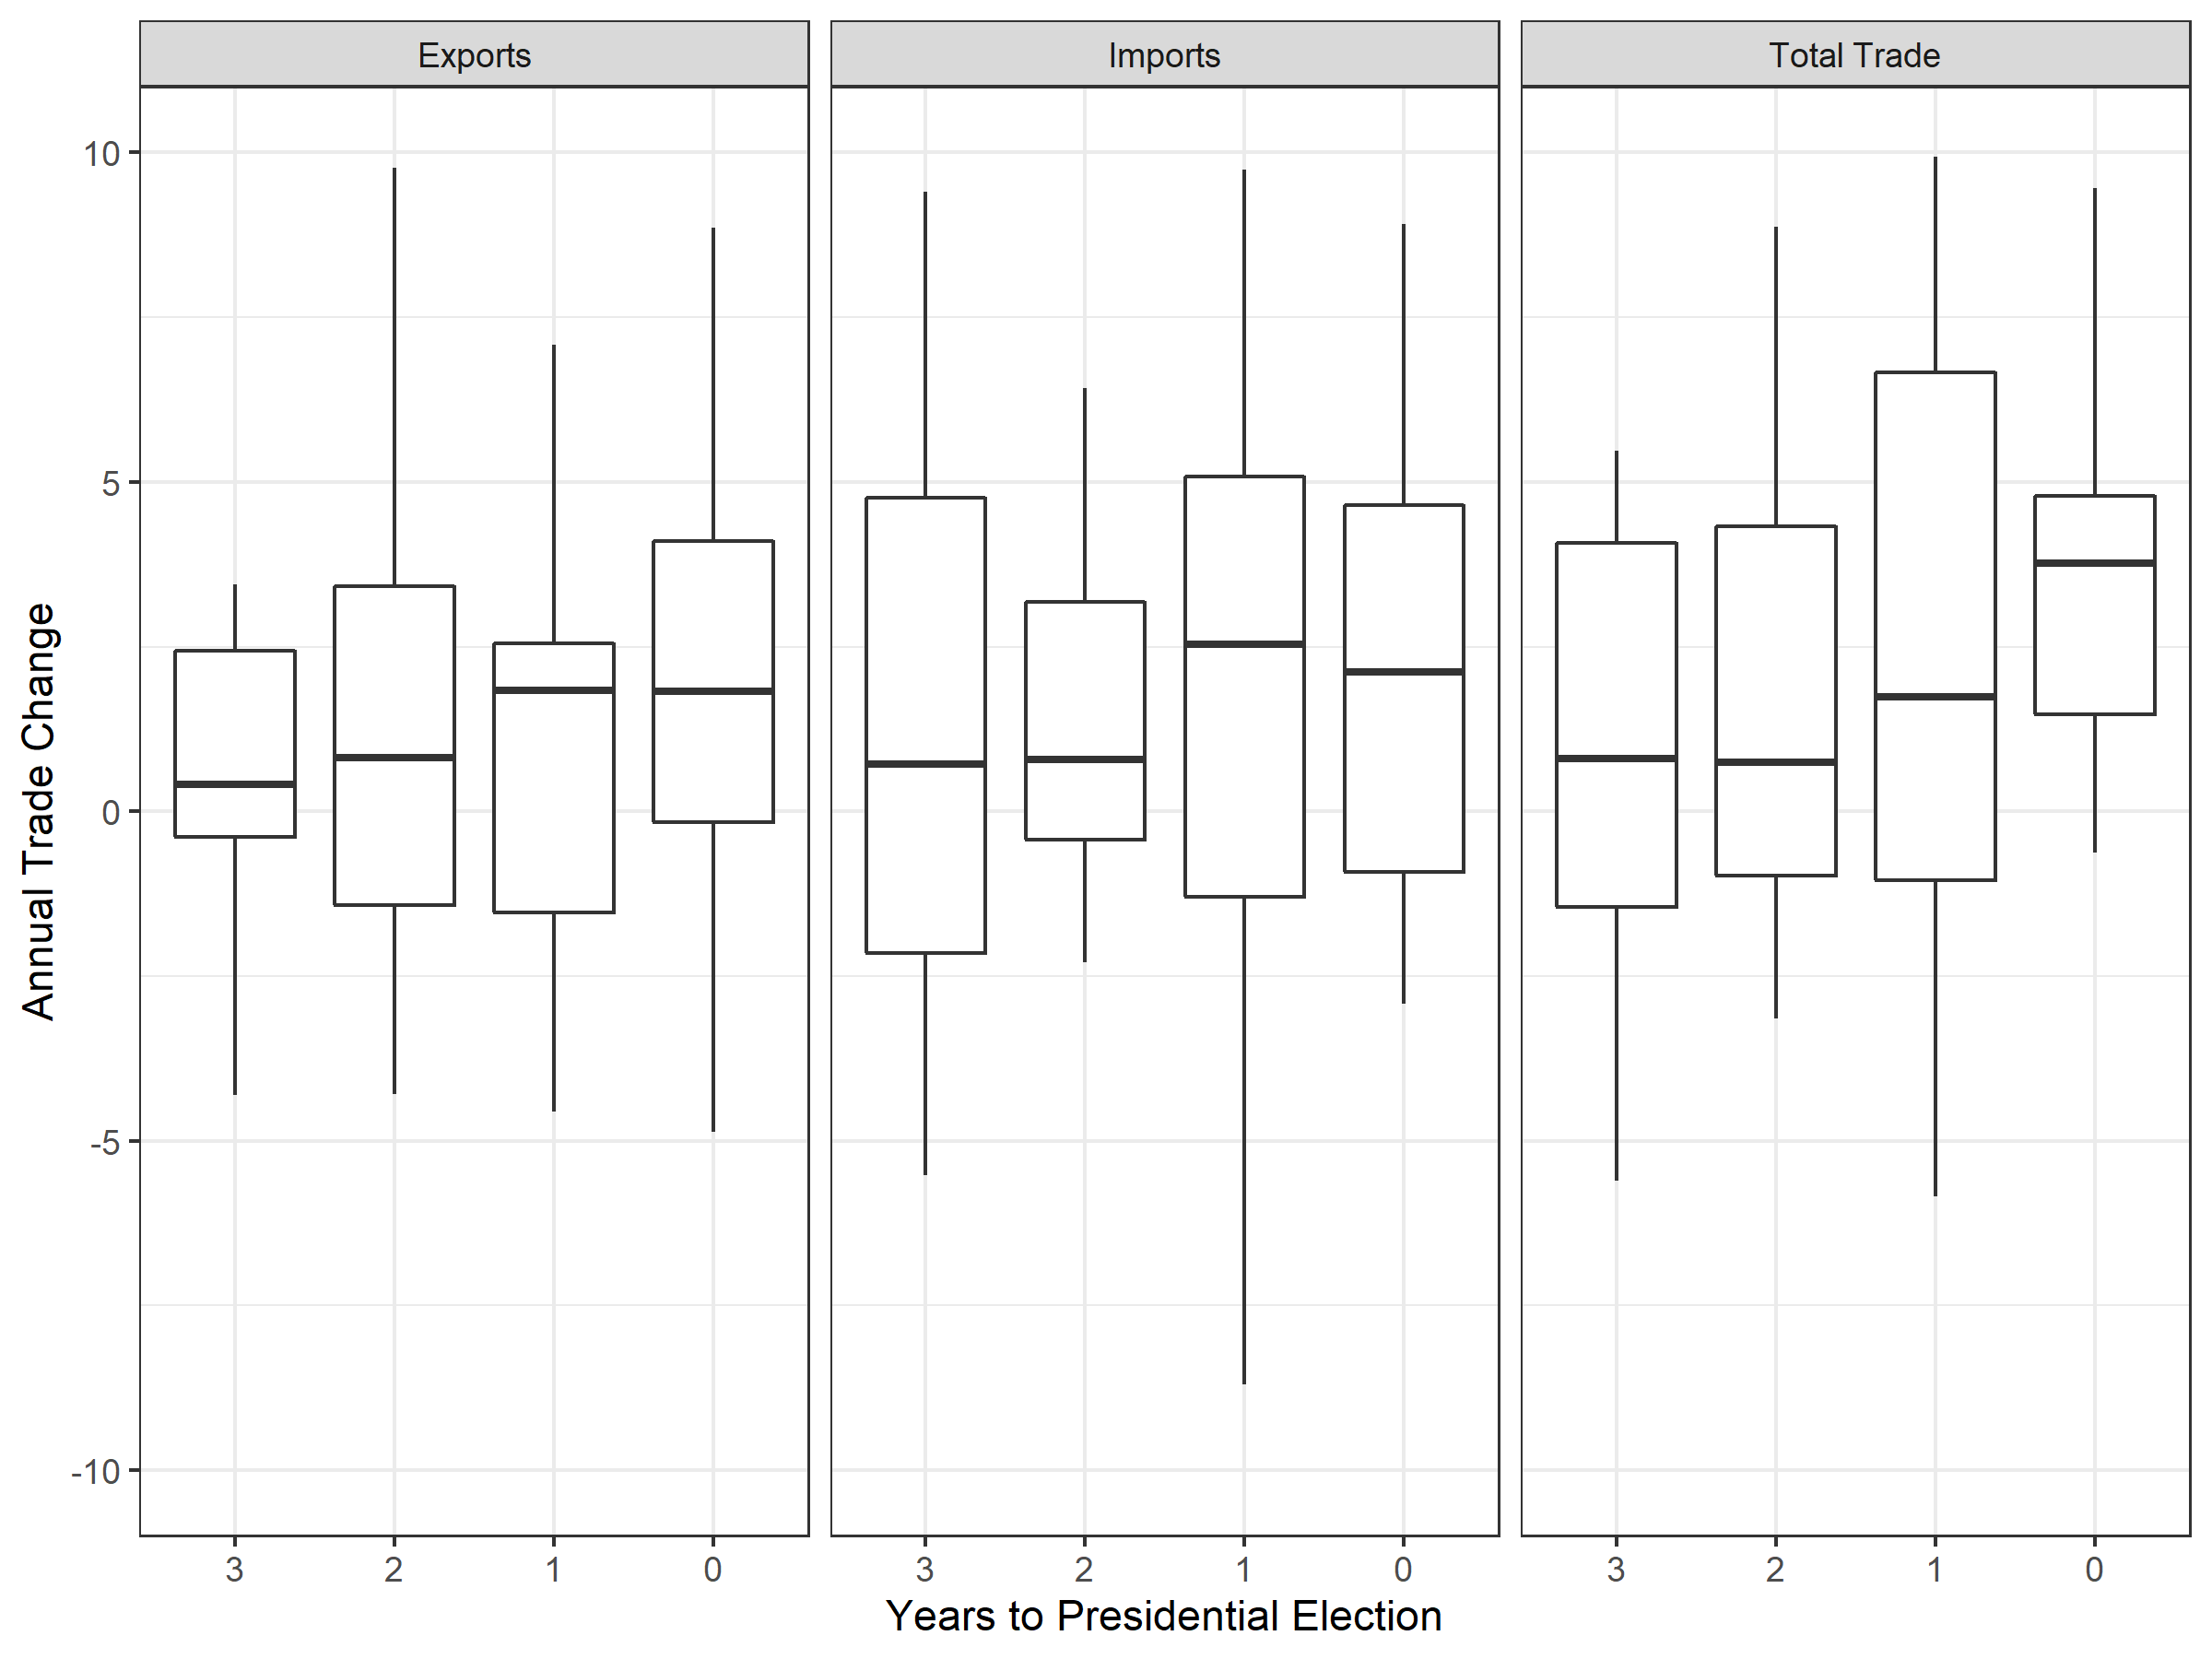
\includegraphics[width=0.95\textwidth]{../figures/us-trade-cycles.png}
\caption{Electoral cycles in U.S. trade between 1951 and 2019. Each box plot summarizes the distribution of changes in logged exports, imports, and overall trade as a presidential election approaches. The thick black line in each plot marks the median value.}
\label{fig:us-trade-cycles}
\end{figure}


While there is ample variation in export changes across, the median export change is highest in the year before or year of a presidential election.
Import changes also rise, though they vary more before an election. 
As a result of increasing exports and imports, total trade changes also increase, especially in presidential election years.


% targeted and flexible policies 
In addition to these general economic roots of electoral trade cycles are straightforward, electoral export cycles require further scrutiny for two reasons.
First, monetary policy is the most likely driver of export cycles, as currency devaluation makes exports more competitive. 
But while \citet[pg. 247]{Dubois2016} notes that independent central banks engage in some cyclical behavior, independence makes monetary policy cycles weaker \citep{ClarkHallerberg2000}. 
Given strong independence at the Federal Reserve, the strong export cycles in \autoref{fig:us-trade-cycles} need additional explanation. 


Both Lyndon Johnson and Donald Trump found major limits to their ability to browbeat Federal Reserve Chairs into changing monetary policy, to give two examples. 
Johnson sought looser monetary policy before the 1968 presidential election, but Fed Chair William McChesney Martin continued to tighten policy.
Trump's tweeted demands for looser monetary policy to increase growth before the 2020 election similarly had little impact on Jerome Powell. 


Second, recent scholarship highlights specific policy cycles because leaders struggle to manipulate aggregate economic instruments where they have more direct influence. 
In fiscal policy, aggregate budgets often give leaders limited spending discretion, which leads to targeted spending shifts \citep[pg. 248]{Dubois2016}.\footnote{This does not rule out fiscal cycles, however.} 
Leaders also employ other policies such as trade disputes \citep{Conconietal2017}, labor agreements \citep{Ahlquist2010} and land reform \cite{Philips2020} to win support in key constituencies.


% Defense spending/contracts as flexible instrument
Many observers believe defense spending is a useful instrument for budget cycles (e.g. \cite{Tufte1978, Mintz1988}).
Executive leaders often have more discretion in defense resource allocation, and defense spending has economic ramifications.
\citet{WhittenWilliams2011} note that defense spending can serve social welfare goals and \citet{Becker2021} finds that unemployment in NATO members encourages leaders to shift spending from equipment to personnel.


% in US context, contracts
Recent studies in the United States argue that defense budgets, which Congress sets two years ahead, are poor political cycle tools, however.
This shifted attention towards defense contracting, as leaders control contract timing and disbursement \citep{Mayer1995, DerouenHeo2000}.
Giving contracts also allows leaders to target key constituencies in response to unemployment and approval shifts by claiming credit for awards \citep{DerouenHeo2000}. 


% increased production of arms- not tied to security needs
Electoral cycles in defense contracting could explain electoral export cycles.
Defense contracting increases arms production by employing firms to produce defense goods. 
While these goods can equip the U.S. military, electoral cycles and defense planning may diverge.
Even the U.S. military may lack absorption capacity to incorporate defense contracting outputs.
Put differently, increased supply from electoral cycles in defense contracting does not respond to increased military demand, requiring other buyers. 
Foreign markets provide alternative outlets for new arms production from defense contracting cycles. 
When contracting cycles produce new goods, U.S. leaders can also sell or transfer old equipment to partners to make room.


% timeline and intermediate goods
Production times for defense goods vary widely.
Large platforms like ships, tanks and airplanes can take years to assemble. 
Still, if foreign states place orders for these platforms near elections, contracts can go out immediately.
Other goods such as small arms, ammunition and missiles, may be produced and exported more quickly. 
Intermediate goods, such as F-35 components, are also exported. 


% additional production and foreign markets
%When defense production and planning diverge, foreign markets provide alternative takers for excess arms production from defense contracting cycles. 
Not all states are equally likely to receive arms exports near elections, however. 
U.S. allies are more likely to take arms exports than other states. 
Security partners are a pivotal outlet because alliances facilitate security, economic and political cooperation.
The United States often transfers or sells arms to alliance proteges, and proteges have means and motivation to accommodate electoral cycles. 



\subsection{Alliances and U.S. Arms Exports}


% basic asymm alliance framework
In asymmetric alliances between large and small states, the large state protects its smaller partner in exchange for foreign policy concessions \citep{Morrow1991}.
A credible promise of military support increases the large state's foreign policy influence. 
Small alliance members garner protection from external threats and sacrifice some foreign policy autonomy. 
%Although many asymmetric alliance formalize hierarchical relationships, security and economic hierarchy are distinct \citep{Lake2009}. 


%Military alliances and economic cooperation are inseparable.
Many alliances also include explicit or implicit promises of economic cooperation \citep{GowaMansfield2004, LongLeeds2006, Davis2008, Poast2012}.\footnote{Conflict and economic integration are linked in general (see for example, \citep{GartzkeLi2003, Chen2021}).}
Prior research indicates that alliances promote trade \citep{Gowa1995, GowaMansfield2004, Haim2016} or protect existing trade ties \citep{Fordham2010}.
Alliances also encourage foreign direct investment \citep{LiVashchilko2010} and monetary cooperation \citep{Li2003}.
A cooperative bargain of security and economic cooperation results. 


% potential markets: allies
% take new or used stuff to make room
Bundles of security and economic cooperation makes U.S. allies an obvious market for outputs from political cycles in defense contracting.
\citet{Thurneretal2019} find that while the relative importance of security and economic factors fluctuates, alliances consistently increase arms transfers.
Common security interests and economic integration of defense industries create economic and security ties that encourage arms trade \citep{Bitzinger1994}. 
Defense industry integration generates trade in intermediate defense goods \citep{Brooks2005}. 


% less export cycles to non-allies
% each evidence sentence could be its own paragraph 
Allies are more likely than other states to receive arms transfers around elections.
The security externalities of arms transfers constrain electoral cycles in arms exports to non-allies. 
U.S. leaders will be less willing to increase the capability of potential opponents, even if it facilitates electoral cycles.
Furthermore, arms transfers outside of alliances could face greater opposition scrutiny near elections, leading presidents to forestall criticism by forgoing contentious transfers.
Limited defense industry cooperation also constrains exports outside alliances to finished goods, while allies with defense industrial ties can receive intermediate goods.


% sending arms: political benefits for patron and proteges
Moreover, electoral cycles in arms exports to allies benefit U.S. and allied leaders.
Presidents gain capacity to manipulate economic conditions with defense contracting and signal support for U.S. alliance proteges by sending arms.
Defense contracting cycles increase prosperity in key electoral areas, which increases a leader's odds of winning office for themselves or their party. 
As for signaling support, \citet{McManusYarhi-Milo2017} argue that arms transfers are a costly but less visible signal of patron support.\footnote{\citet{Yarhi-Miloetal2016} argue that arms transfers sometimes substitute for alliances so patrons can provide security with less entrapment risk.}


% positive statecraft tie-in from Baldwin 
Allied leaders also benefit from arms exports around elections, because arms exports curry favor with an alliance patron, bolster military capabilities and deepen perceived commitment.
Helping patron leaders by receiving arms will dispose the more favorably towards an ally. 
Allies increase their military capabilities with new arms as well, which can make their fighting forces more effective. 
Finally, because arms transfer are a costly support signal \citep{McManusYarhi-Milo2017}, allies gain greater confidence that their patron has made a credible commitment. 


Accepting arms exports is therefore positive economic statecraft. 
Purchases and transfers are a common way that states bolster their political influence \citep[pg. 42-3]{Baldwin2020}.
In alliance politics, \citet[pg. 184-5]{IkenberryGrieco2003} note that states often use direct transfers to attract and sustain security commitments.  


Allied leaders have clear motives to take arms exports, and they also have sufficient political means. 
Arms transfers fall under direct leader control, which gives allies flexibility to respond to U.S. defense contracting cycles.
Arms imports are more flexible than tariffs or other trade policies that leaders could manipulate to boost trade with the United States.
Governments are the customer for most arms sales or transfers, so they have more latitude to take arms.
Direct control over these decisions mirrors how political control of firms increases trade policy flexibility \citep{Davisetal2019}.


% Sales and transfers- who pays for what
Moreover, proteges do not always pay for U.S. arms transfers.
The United States often subsidizes or gifts arms transfers through foreign military sales programs. 
While these still count as arms exports, they impose few immediate costs on recipients.
Alliances make such subsidized transfers to allies easier for presidents to justify to other elites, as they promote common security interests. 


% deliberate or not? 
This argument is agnostic about whether allies make a conscious decision to help political budget cycles by taking arms exports.
U.S. allies need not make deliberate choices to accommodate electoral cycles in defense contracting, they may receive better terms and more financial support to take additional goods. 
Allies could also take transfers or surplus materiel as a deliberate favor to leaders who have supported their foreign policy interests, however. 


The overall argument process is as follows.
First, budget cycles increase defense contracting awards and drive import cycles by increasing economic growth. 
Greater defense contracting increases arms production, which then augments arms exports to allies.
The import side of this process depends on foreign firms meeting increased domestic demand.
\autoref{fig:arg-process} summarizes this sequence.


\begin{figure}[htpb]
\adjustbox{scale = .90}{
\centering
\begin{tikzcd}[ampersand replacement=\&]
                                                   \& |[alias=Gr]| \mbox{Econ. Growth}   \arrow[r]  \&  \mbox{Imports from Firms} \arrow[r]  \&  |[alias=Y]| \mbox{Trade Cycles}   \\
\mbox{Budget Cycles} \arrow[bend left = 10, to = Gr] \arrow[r]  \& \mbox{Defense Contracting} \arrow[r] \& \mbox{Arms Production} \arrow[r] \& \mbox{Arms to Allies} \arrow[u]  
\end{tikzcd}
}
\caption{Summary of the argument process.}
\label{fig:arg-process}
\end{figure}


%\begin{table}
%\resizebox{.99\textwidth}{!}{
%\begin{tabular}{ccccccc}
%\mbox{Budget}  & $\rightarrow$    & \mbox{Defense}     & $\rightarrow$ & \mbox{Arms}     & $\rightarrow$ & \mbox{Trade Cycles, especially} \\
%\mbox{Cycles}  &                  & \mbox{Contracting} &               &  \mbox{Production}   &               & \mbox{Arms to Allies} \\
%\end{tabular}
%}
%\end{table}


% Net implications: total trade increases and trade balances unchanged
Given defense contracting cycles, I expect greater exports to allies through arms transfers around U.S. elections.
Imports will also contribute to greater total trade around elections, but imports depend on firms decisions and thus be less responsive to security cooperation.
The relative impact on trade balances depends on whether imports or exports increase more. 
If U.S. proteges take more exports than non-allies, the U.S. trade balance with those states will improve relative to trade balances with non-allies however.


% Result- increased exports, tied to electoral cycles
The result of this process is increased trade as elections approach, especially exports from the United States to alliance proteges.
Electoral export cycles in alliances reflect trade in arms and intermediate defense goods. 
Arms exports in turn are rooted in electoral cycles of defense contracting.



\subsection{Implications}



The argument generates several testable implications, within specific scope conditions. 
Cycles are most likely in states with a large economy, alliance partners and a robust domestic defense industry. 
Fixed election scheduling further reduces endogeneity between policy decisions and strategic election timing.
Therefore, the argument and analysis focus on the United States. 
Other states may have weaker cycles, or electoral cycles in different goods.


The first hypothesis predicts general electoral cycles in trade, especially exports to allies. 
As presidential elections approach, I expect greater imports and increasing exports from the United States to alliance proteges.


\begin{quote}
\textsc{Trade Cycles Hypothesis: As time to a presidential election decreases, U.S. imports and exports will increase, and exports to allies will increase more than exports to non-allies.}
\end{quote}



The second hypothesis predicts corresponding cycles in arms exports.
If arms transfers and sales drive export cycles, we should observe corresponding electoral cycles in arms transfers.
Proximity to presidential elections will increase arms transfers from the United States to allied states. 


\begin{quote}
\textsc{Arms Exports Hypothesis: As time to a presidential election decreases, U.S. arms exports to allies will increase.}
\end{quote}


The third prediction tests the expected relationship between defense contracts and arms exports. 
I expect electoral cycles in defense contacting, and a positive correlation between these cycles and U.S. arms exports.


\begin{quote}
\textsc{Defense Contracts Hypothesis: As defense contracting increases around elections, U.S. arms exports will increase.}
\end{quote}


% TODO(Josh): Rework this totally
In the following, I describe how I scrutinize each of these hypotheses. 
In the first analysis, I establish the role of allies in electoral export cycles. 
The second analysis shows increasing exports to allies track with the U.S. electoral cycles, and are of comparable magnitude to trade cycles.
Finally, I offer a preliminary examination of the final link in the argument with descriptive data on defense contracting from 2000 to 2020, which does not fully test the defense contracts hypothesis.




\section{Electoral Cycles in U.S. Exports to Allies}

To test the first hypothesis, I analyze U.S. trade from 1950 to 2014. 
This analysis establishes that allied states see larger electoral export cycles than non-allies, while U.S. imports increase regardless of security ties. 
The key independent variable measures years until a presidential election year.
The years to election variable ranges from zero in election years to three in the year immediately after an election. 
The second key variable is a dummy indicator of a defensive alliance between the United States and each state, drawn from the ATOP database \citep{Leedsetal2002}.
%employ elections data from the National Elections across Democracy and Autocracy (NELDA) dataset \citep{HydeMarinov2012} to
Finally, I interact the defensive alliance dummy with the years to election variable.


The key outcomes are annual changes in the natural log of exports, changes in log imports, changes in total trade, and trade balance changes.
The total trade changes and trade balance changes measures assess the net impact of export and import changes.
I use changes because models in levels with a lagged dependent variable suggest non-stationarity in many panels. 
Lagged trade flows have unit roots or near unit root coefficients, so models in levels risk spurious inferences \citep{GrangerNewbold1974}.
I draw on exports and imports data from the IMF's direction of trade statistics database.


For U.S. exports, my argument makes three predictions about the interaction between alliances and years to election in the exports model. 
First a positive constituent term on the defensive alliance variable, which indicates that allies take more exports than non-allies in election years, when time to an election is zero.
Second, I expect a negative constituent term on years to election as non-allied states respond to political business cycles with increases in other trade. 
Last, a negative interaction between alliances and time to the election would indicate that exports to allies are more responsive to elections than exports to states without a defensive alliances with the United States.


I expect no interaction between alliances and election proximity for U.S. imports, because imports reflect general economic growth.
Foreign firms will respond to increased U.S. demand regardless of alliance cooperation.  
Allies may export more to the United States than other countries, but they will not be more responsive to elections.


In addition to the interaction of time to elections and a defensive alliance, I include a series of control variables that may be correlated with alliances and trade. 
Key trade variables include for changes in the GDP of both states, population-weighted distance, contiguity, common language and former colonial ties \citep{FouquinHugot2016}.
I also adjust for democracy \citep{Marquez2016}, the presence of a militarized interstate dispute \citep{Gibleretal2016}, and shared IGO membership \citep{Pevehouseetal2020}.\footnote{Some dyadic data from the \textit{peacesciencer} \textsf{R} package \citep{peacesciencer-package}.}


Some trade flow changes are unusual. 
This creates heavy-tailed residuals, so I employ a robust regression estimator; M-estimation with Tukey's biweight function \citep{RaineyBaissa2020}.
Robust regression places less weight on unusual observations, making it more efficient than OLS for this particular outcome.



\subsection{Results}


Raw trade data shows differences between allies and non-allies for electoral cycles in U.S. exports, imports and total trade. 
\autoref{fig:us-trade-cycles-all} presents the distribution of changes in logged exports, imports and overall trade in years with differing proximity to presidential elections.
Box plots summarize the distribution of U.S. trade with all states in those years. 
The dark line in each box plot marks the median value. 


\begin{figure}
\centering
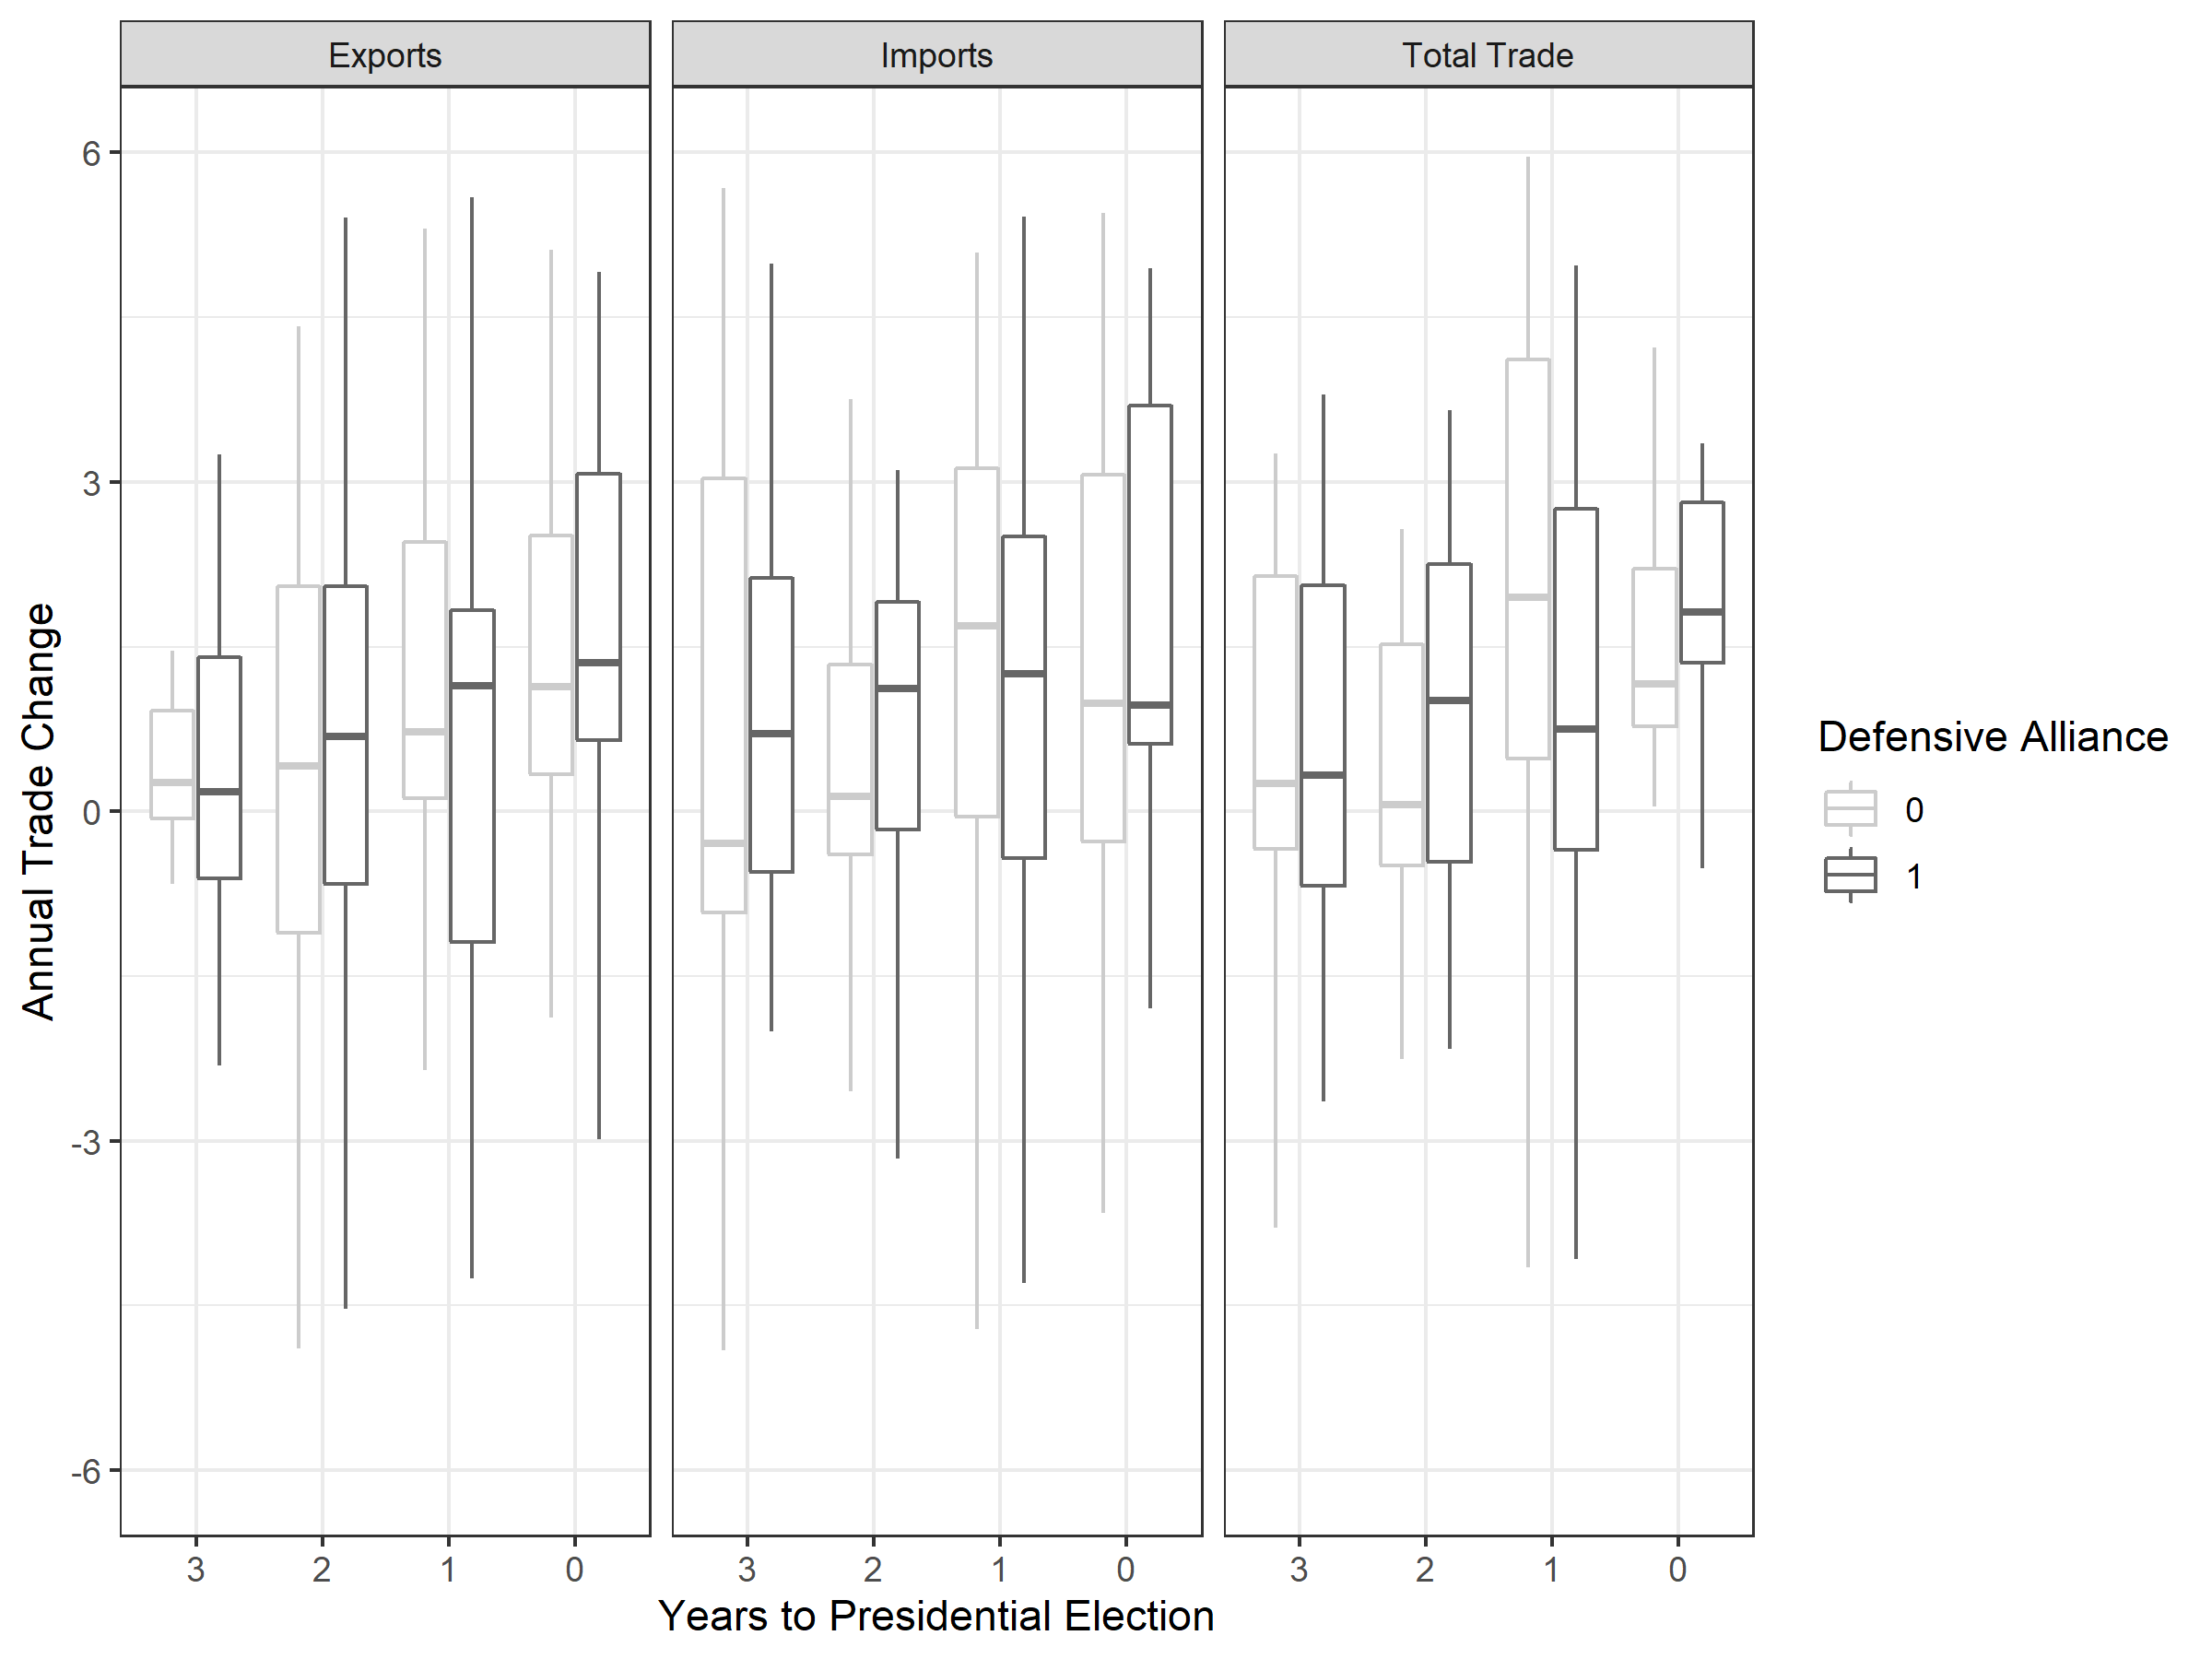
\includegraphics[width=0.95\textwidth]{../figures/us-trade-cycles-all.png}
\caption{Electoral cycles in U.S. trade between 1950 and 2014. Each box plot summarizes the distribution of changes in logged exports, imports, and overall trade as a presidential election approaches. Colors mark trade with allies and non-allies. The thick black line in each box plot marks the median value.}
\label{fig:us-trade-cycles-all}
\end{figure}


Median export changes are higher for allies than non-allies near presidential elections. 
Export changes for non-allies still rise, but less than exports to allies. 
Imports from non-allies and allies are equally responsive to election timing. 
As a result, total U.S. trade increases regardless of formal security ties.


\autoref{fig:us-trade-cycles} shows electoral cycles in U.S. trade, but it is possible that other factors confound this relationship.
\autoref{fig:us-trade-coefs} presents coefficient estimates from the robust regression models of the four trade outcomes, along with 95\% confidence intervals. 
These estimates suggest that allies receive substantial U.S. export cycles, but all states respond to elections with increased exports to the United States. 


\begin{figure}
\centering
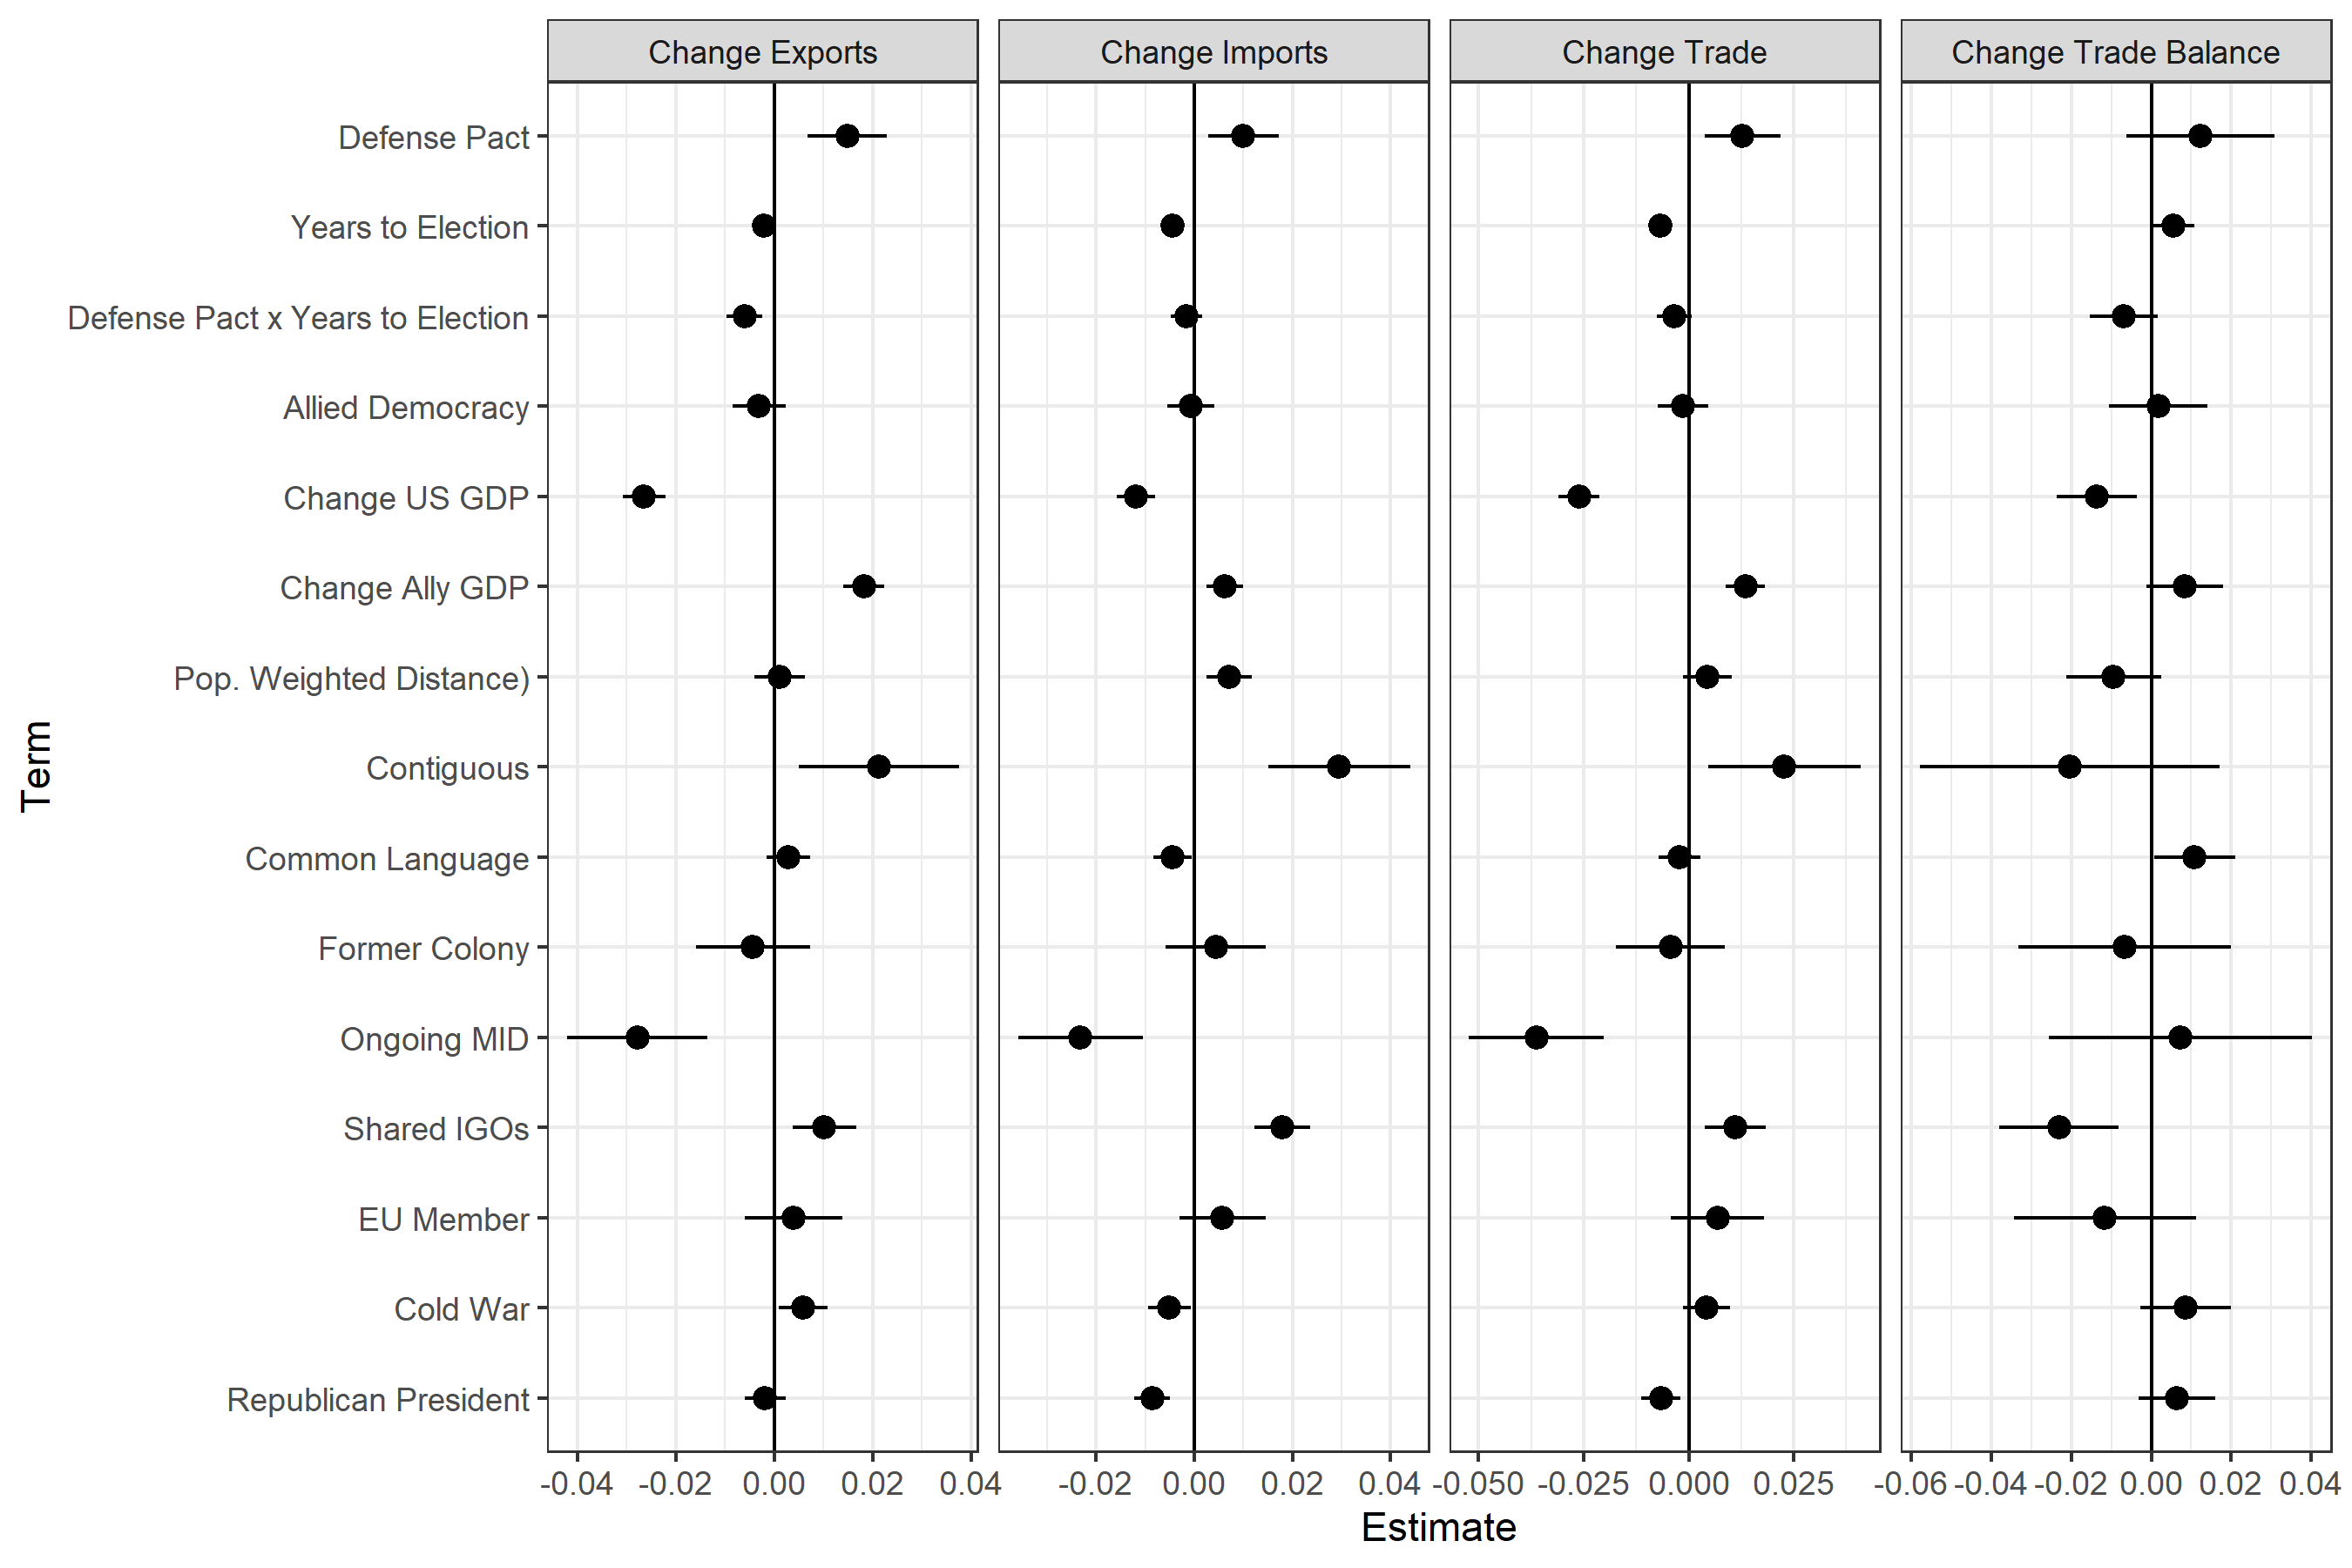
\includegraphics[width=0.95\textwidth]{../figures/us-trade-coefs.png}
\caption{Robust regression coefficients from models of U.S. trade, 1950 to 2014. Points mark coefficient estimates and error bars encapsulate 95\% confidence intervals. All continuous predictors rescaled by two standard deviations.}
\label{fig:us-trade-coefs}
\end{figure}


As expected, the interaction between the defensive alliance dummy and years to election is negative in the exports model, which implies that allies receive more U.S. exports as presidential elections approach.
Allies receive more U.S. exports in election years, and respond especially strongly to election timing.
The smaller constituent term on the election years constituent term in the exports model implies a smaller electoral cycle in exports to non-allies.


The interaction term for imports suggests no clear difference in U.S. imports around elections between allies and non-allied states. 
Moreover, the time to election constituent term is negative for all outcomes, except the trade balance. 
This is indicative of similar electoral cycles between allies and non-allies.
Trade changes approximate the track of exports. 
Simultaneous increases in imports and exports have an unclear impact on trade balances, however. 
 


% predicted
The sign and confidence intervals of the interaction terms are inadequate evidence of a conditional relationship \citep{BramborClarkGolder2006}, so I plot predicted changes in trade flows in \autoref{fig:us-elec-pred}.
This figure presents predicted changes in trade across time to election for states with and without a U.S. defense pact. 
Given non-linear relationships from logged trade flows and a robust estimator, these predictions are more straightforward to interpret than marginal effects.\footnote{I present marginal effects in the appendix.} 


\begin{figure}[htpb]
	\centering
		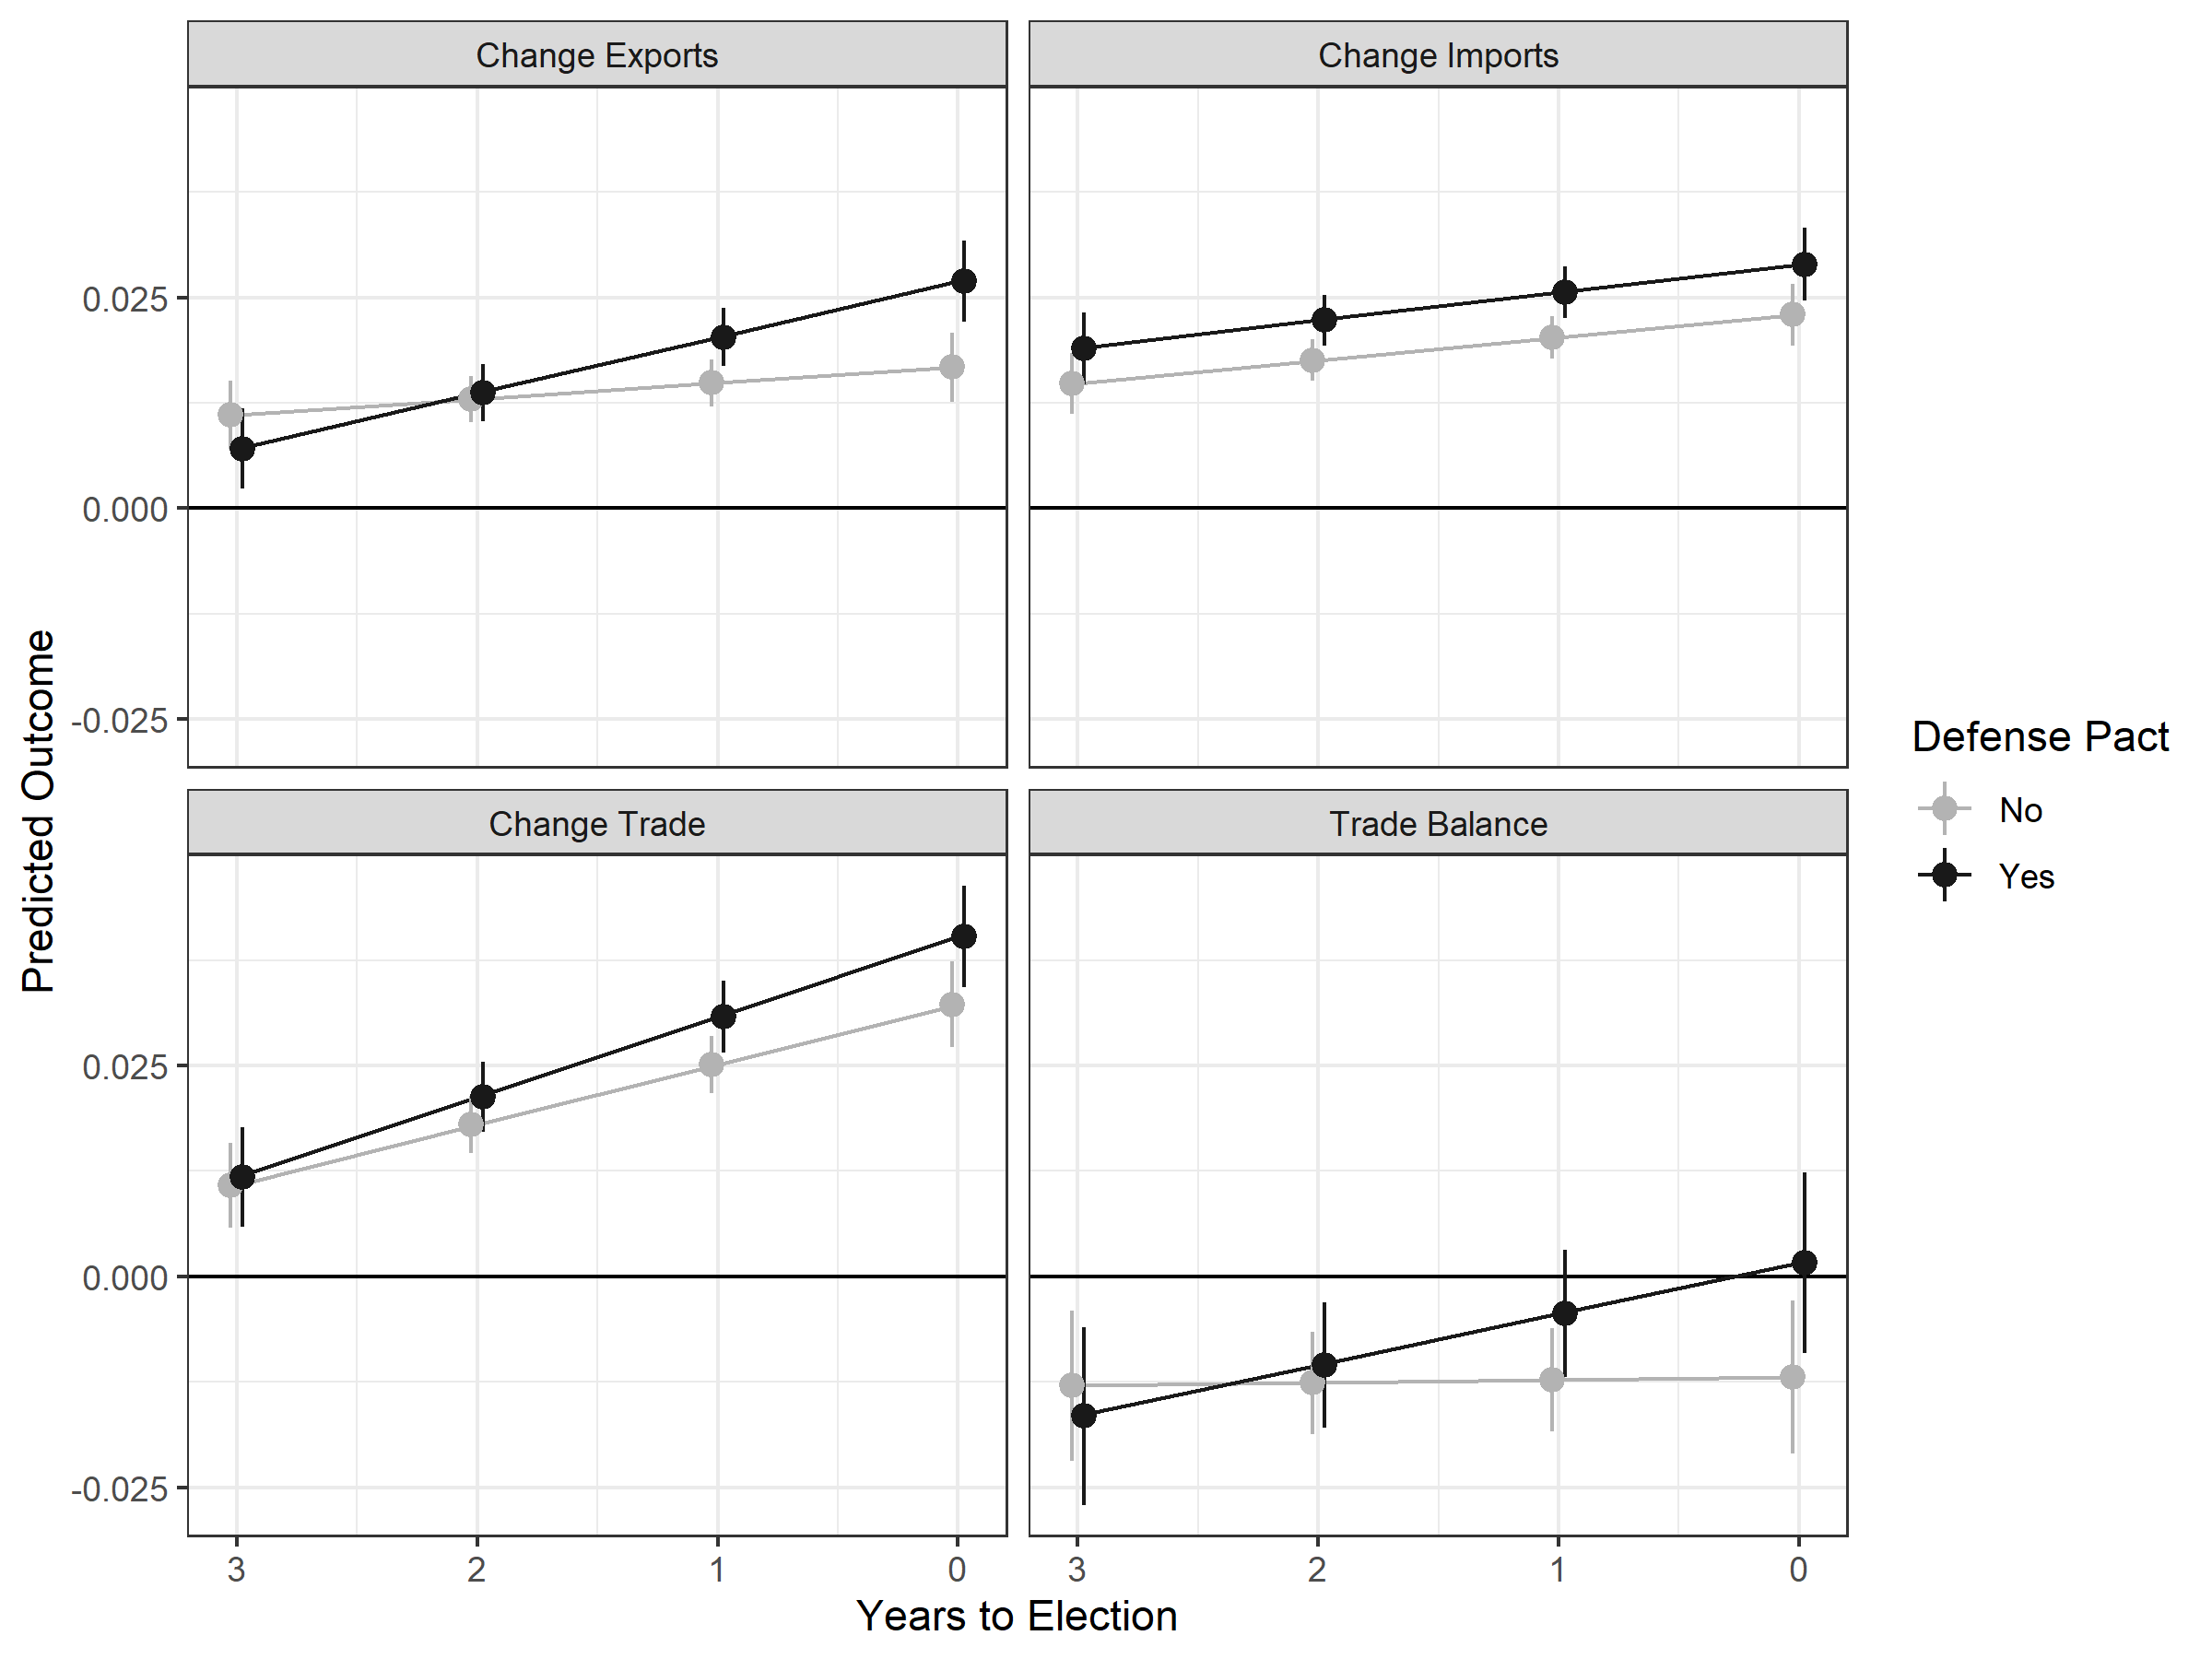
\includegraphics[width=0.95\textwidth]{../figures/us-elec-pred.png}
	\caption{Predicted changes in trade between the the United States and other states. Points mark the predictions and error bars summarize the 95\% confidence interval.}
	\label{fig:us-elec-pred}
\end{figure}


Predicted changes in exports, imports, total trade and the trade balance are consistent with inferences from the coefficient estimates. 
While U.S. exports to non-allies rise somewhat with election proximity, exports to allied states increase more. 
Allied and non-allied export changes are comparable until the year before and year of U.S. presidential elections, and after that, exports to U.S. allies increase by far more. 


% time to election
U.S. imports increase as presidential elections approach, and there is little difference in the trend between allies and other states. 
This is the result of political budget cycles boosting domestic consumption, which do not target specific goods.
Imports from allies are consistently greater than imports from non-allies, however, which is consistent with prior work on alliances and trade promotion \citep{GowaMansfield2004}. 


Differences in exports produce distinct electoral trade cycles between states with a U.S. defense treaty and those without. 
Non-allies increase imports and exports in similar ways as elections approach. 
As a result, their total trade changes increase with election proximity, but less so than allies. 
Allied trade with the United States rises more than trade with other states in presidential election years. 


Trade balances, a key concern for some policymakers, show less evidence of electoral cycles. 
U.S. trade deficits with allies narrow somewhat around elections, but expand with non-allies, as imports rise more than exports. 
Uncertainty estimates makes distinguishing predictions between and within the two groups difficult.


% improved trade balance
These results are consistent with the export cycles hypothesis. 
Exports to allies increase more near elections than exports to non-allies.
In the next section, I show that differences in arms transfers to allies track electoral export cycles.



\section{Arms Transfers and Presidential Elections}


I model U.S. arms transfers from 1951 to 2014 using data from the SIPRI Arms Transfer Database \citep{SIPRI2021}.
The outcome in this analysis is annual logged arms transfers, based on SIPRI's trend indicator value methodology for major conventional weapons.
I model arms transfer levels because these shifts are less autocorrelated than overall exports.
I cannot use the same estimation strategy, however, because 60\% of the observations have zero observed arms transfers.
Such zero-inflation makes standard regression techniques inefficient.
To overcome this issue, I use a two-stage model to approximate a hurdle into non-zero arms transfers. 


In the first stage, I model a binary indicator of non-zero arms transfers with a logistic regression. 
The logistic regression predicts U.S. arms transfer presence with the defensive alliance dummy, dummy indicators of the Cold War, EU membership and Republican presidencies, recipient democracy, shared IGO membership and MID participation. 
I also include indicators of U.S. and recipient GDP, population-weighted distance, along with binary measures of common language, contiguity and colonial history. 
Finally, I account for duration dependence with cubic time polynomials \citep{CarterSignorino2010}.


The second stage model is a linear regression of all non-zero arms transfers.
This model of arms transfers adjusts for the predicted probability of non-zero arms transfers and a lagged arms transfer indicator to the predictors from the model of changes in exports.
As in the trade models, I interact defense pacts and time to election to capture differences in electoral cycles between U.S. allies and non-allies. 
Other controls match the exports model, encapsulating economic, cultural, and distance in ties between the United States and other states. 
As a result, the overall approach approximates a hurdle from zero to positive arms transfers in modeling U.S. arms exports. 


\subsection{Results}


These results proceed in two parts.
First, I present the coefficient estimates from the logistic regression of arms transfer presence and regression of arms transfers on election proximity and alliances in \autoref{fig:us-trade-cycles}.
I then summarize the interaction of alliances and presidential election proximity in \autoref{fig:us-arms-plots}.


At the arms transfer hurdle stage, defense pacts increase the likelihood of any arms transfer, as does contiguity, shared IGO membership, and former colonial ties.
Increasing partner GDP increases the likelihood of arms transfers.
More distant states are also more likely to receive arms transfers, as the United States sells many arms outside the Western Hemisphere. 
After accounting for alliances, increasing democracy and U.S. GDP make arms transfers less likely, as did the Cold War. 
The negative Cold War coefficient reflects dispersion in U.S. arms transfers across more states after the USSR collapsed.


\begin{table}
\centering
\resizebox{\textwidth}{!}{
\begin{tabular}[t]{lcc}
\toprule
  & Non-Zero Arms Transfer: Logit & Arms Transfers: OLS\\
\midrule
Defense Pact & 1.61 & 0.34\\
 & (1.43, 1.79) & (0.13, 0.56)\\
Years to Election &  & 0.04\\
 &  & (-0.02, 0.10)\\
Defense Pact x Years to Election &  & -0.08\\
 &  & (-0.16, -0.01)\\
Partner Democracy & -0.34 & -0.01\\
 & (-0.51, -0.18) & (-0.12, 0.11)\\
US GDP & -0.50 & -0.19\\
 & (-0.76, -0.25) & (-0.37, -0.01)\\
Partner GDP & 0.24 & 0.09\\
 & (0.06, 0.42) & (0.01, 0.18)\\
Pop. Weighted Distance) & 1.39 & 0.49\\
 & (1.23, 1.56) & (0.33, 0.65)\\
Contiguous & 1.12 & 0.59\\
 & (0.53, 1.78) & (0.32, 0.86)\\
Common Language & -0.04 & -0.22\\
 & (-0.17, 0.09) & (-0.31, -0.12)\\
Former Colony & 1.00 & 0.22\\
 & (0.50, 1.54) & (0.04, 0.40)\\
Ongoing MID & -0.81 & -0.20\\
 & (-1.23, -0.40) & (-0.55, 0.15)\\
Shared IGOs & 2.63 & 0.54\\
 & (2.40, 2.87) & (0.25, 0.83)\\
EU Member & -0.20 & -0.30\\
 & (-0.52, 0.14) & (-0.48, -0.12)\\
Cold War & -0.80 & -0.18\\
 & (-1.04, -0.56) & (-0.37, 0.02)\\
Republican President & -0.10 & -0.03\\
 & (-0.23, 0.02) & (-0.12, 0.06)\\
Lag Ln(Arms Transfers) &  & 0.61\\
 &  & (0.58, 0.63)\\
Pred. Prob. of Arms Transfer &  & -0.65\\
 &  & (-1.21, -0.09)\\
\midrule
Num.Obs. & 7879 & 3268\\
\bottomrule
\end{tabular}
}
\caption{Coefficient estimates from a logistic regression of non-zero U.S. arms transfers and robust regression of changes in arms transfers. All continuous predictors rescaled by two standard deviations. Intercepts included but omitted from the table. The logit model estimates also omit the cubic time polynomials.}
\label{tab:arms-ch-hurdle}
\end{table}


In the regression of arms transfer levels, states with a U.S. defense pact receive more arms in presidential election years. 
As with overall exports, the difference between allies and non-allies increases as time to an election decreases.
The key difference with the overall exports finding is that arms transfers to non-allies fall as presidential elections approach. 
This suggests that increasing exports from the United States to non-allies around elections concentrate in other goods. 


Alliances and elections are not the only meaningful predictors of arms transfers.
Arms transfer levels are less sensitive to partner democracy, but increase with allied GDP and decrease with U.S. GDP. 
Contiguous, more distant and former colonial states also receive more transfers, as do states that share more IGO memberships with the United States.
The predicted probability of arms transfer coefficient implies that states that were more likely to receive arms are less likely to see large export increases.  
U.S. GDP growth reduces arms exports. 
The Cold War coefficient is largely negative, perhaps as the scale of arms transfers was more limited in that period. 
Last, there is some temporal autocorrelation in arms transfers, as the lagged dependent variable of .61 shows.


Again, the coefficient estimates in \autoref{tab:arms-ch-hurdle} are imperfect indicators of how alliances and electoral proximity interact.
\autoref{fig:us-arms-plots} therefore plots predicted arms transfers and marginal effect of defense pacts.
These predicted changes in arms transfers and estimated marginal effect of defensive alliances are consistent with the arms exports hypothesis.


\begin{figure}[htpb]
	\centering
		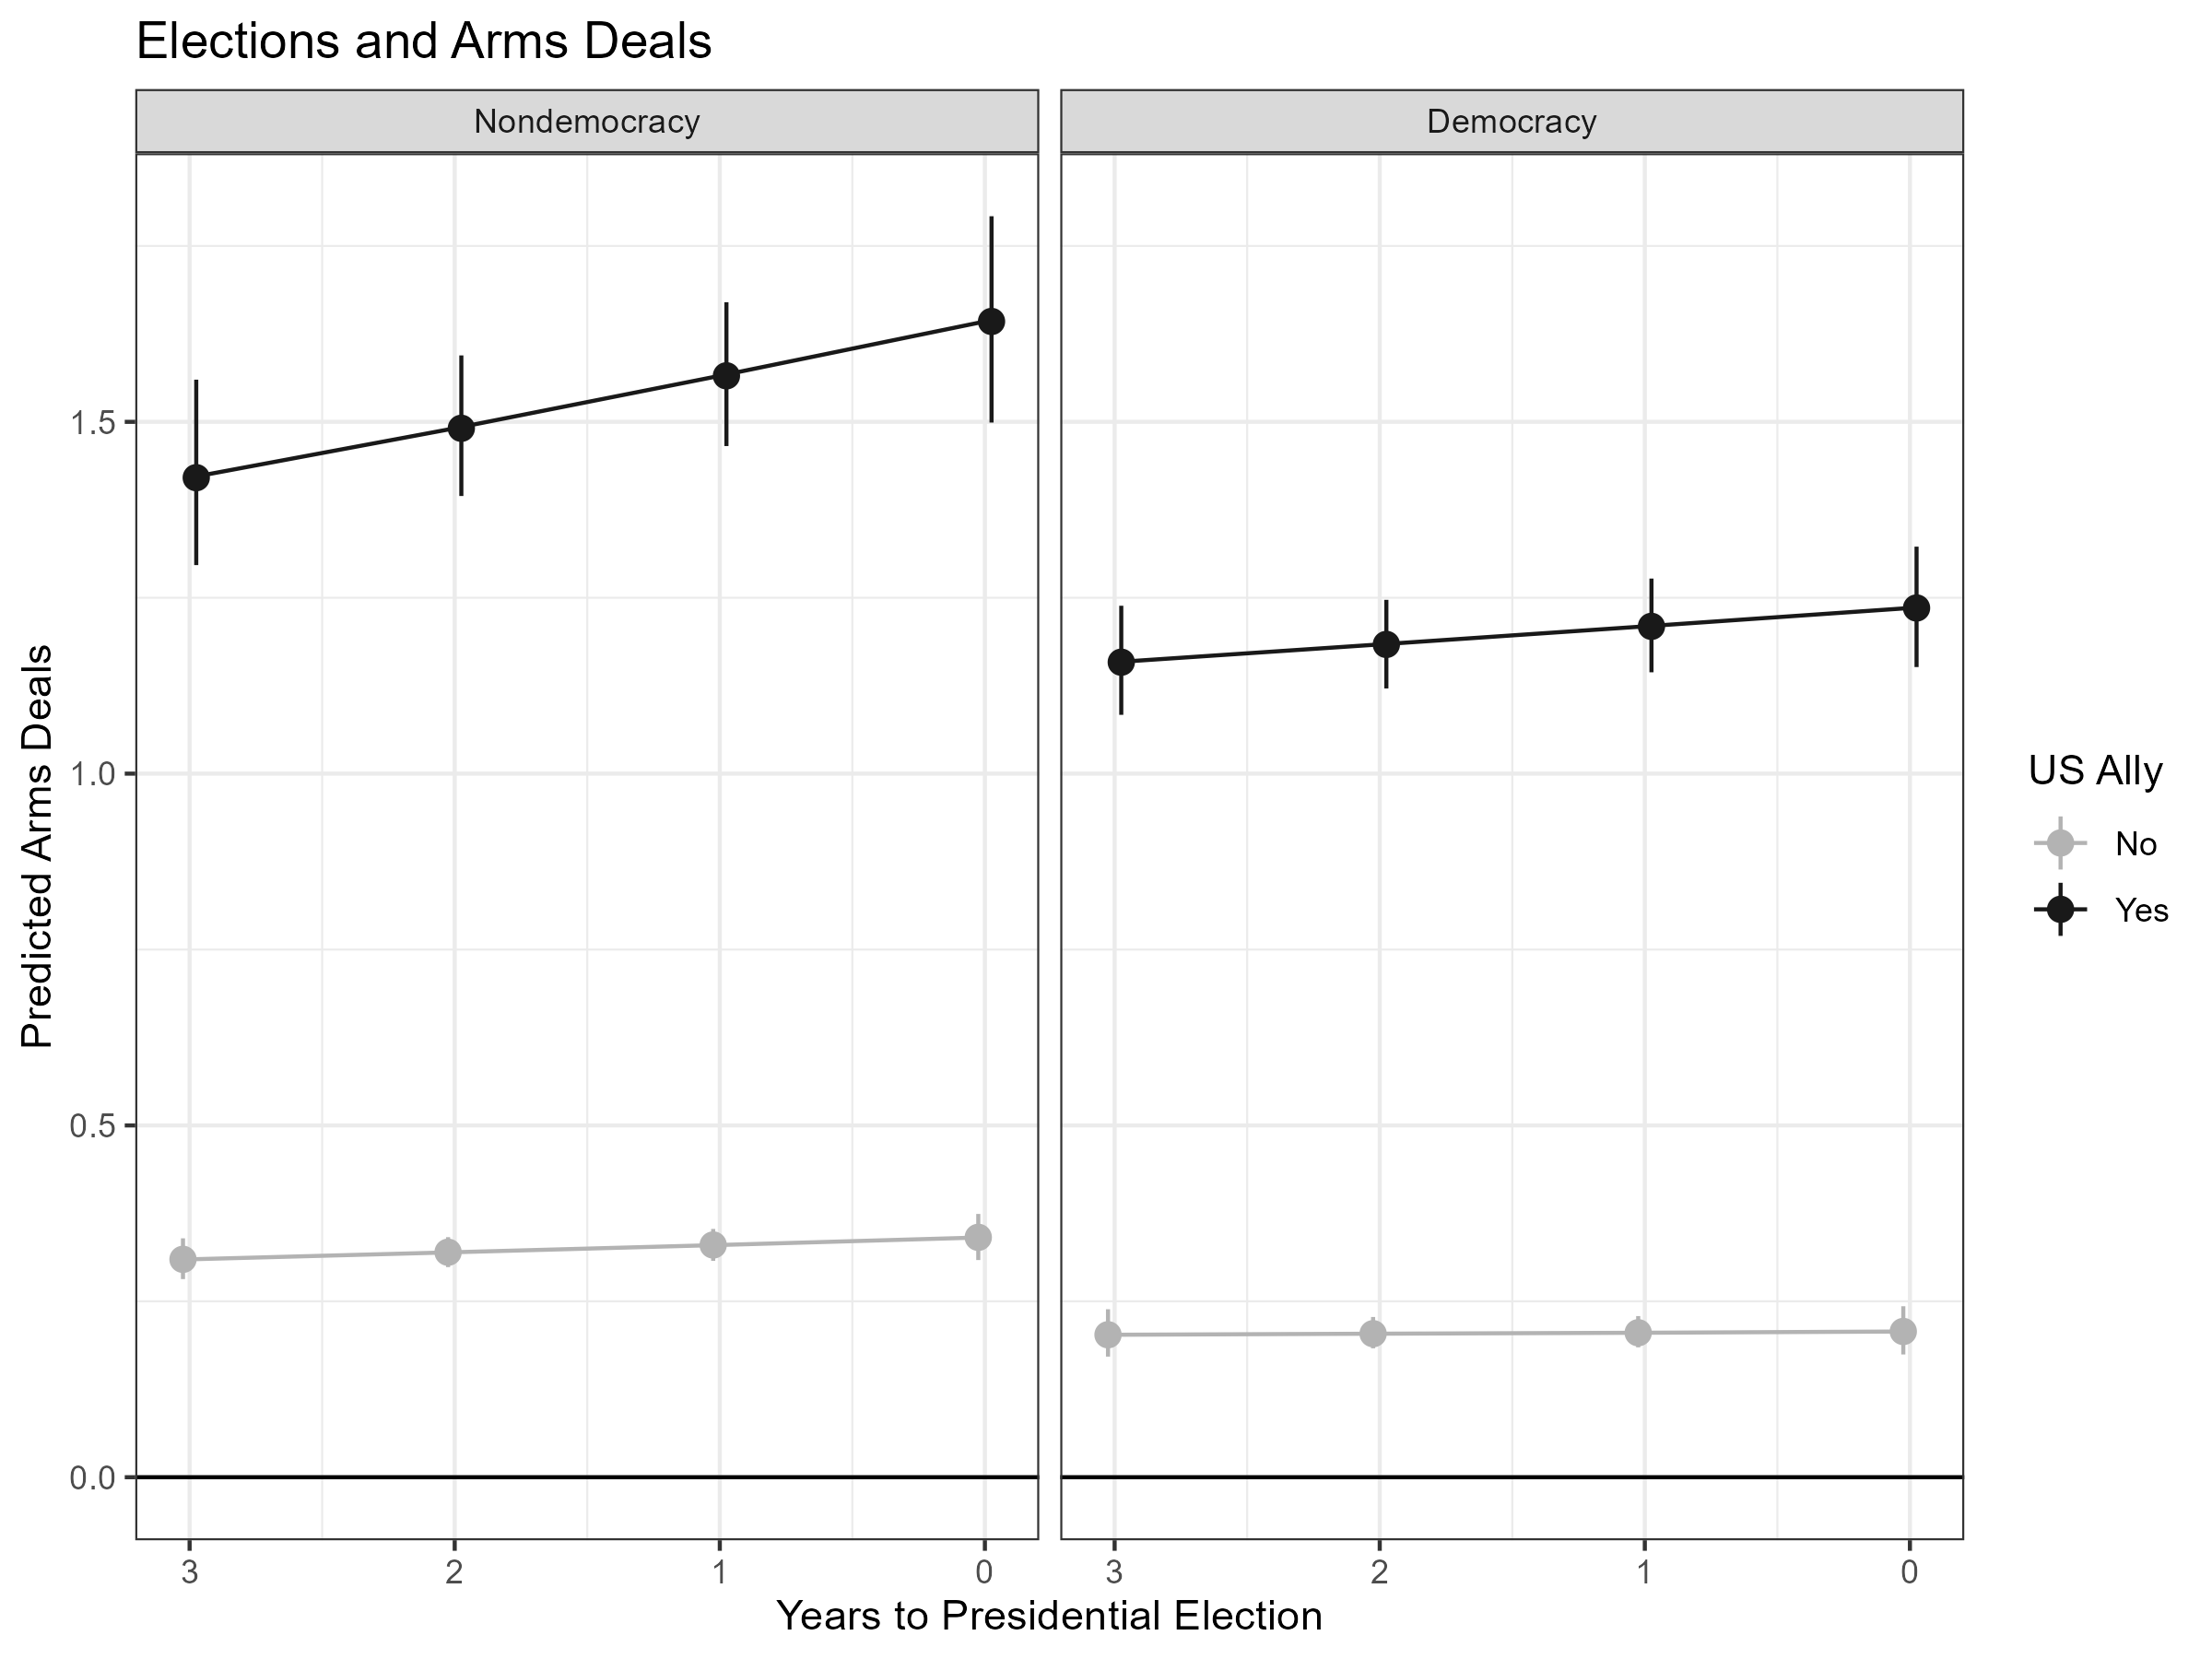
\includegraphics[width=0.95\textwidth]{../figures/us-arms-plots.png}
	\caption{Predicted outcome and the marginal impact of defensive alliances on changes in the log of arms transfers between the United States and other states 1950 to 2014. Points mark the estimates and error bars summarize the 95\% confidence interval.}
	\label{fig:us-arms-plots}
\end{figure}


First, predicted arms transfers to U.S. allies increase as presidential elections approach.
For a U.S. ally, predicted log arms transfers rise by .14 in expectation. 
This is roughly equal to the marginal effect of an alliance on overall exports reflected in \autoref{fig:us-elec-pred}.
At the same time, arms transfers to non-allies fall as elections approach. 


As a result, while arms transfers to allies and non-allies are similar in the year after a presidential election, there is a expected gap of .34 between allies and non-allies in election years.
The marginal impact of a defense pact on arms transfers reflects this difference, as it rises near presidential elections.
U.S. allies thus receive more arms near presidential elections than other states, as security cooperation and defense industry integration encourage arms exports.


Divergent electoral cycles in arms transfers reflect distinct political relations.
Allies have more to gain from accommodating electoral cycles in arms transfers, and can fit additional U.S. arms into military forces that already use U.S. kit.
Arms transfers cement cooperative relationships and bolster allied security through additional capability.
Leaders may also face more scrutiny over arms transfers outside alliances as elections approach. 


These growing arms exports to allies near elections are the result of electoral cycles in defense contracting. 
The next piece of evidence demonstrates the presence of electoral cycles in defense contracting.  
Future iterations of the paper will analyze this final stage of the process more fully. 



\section{Defense Contracting Cycles}


To show electoral cycles in defense contracting, I draw on Department of Defense prime contract award data from the USAspending.gov database.\footnote{Link here: \url{https://www.usaspending.gov/download_center/custom_award_data}.} 
This archive contains data on individual contract awards from to 2000 fiscal year on.
I collected all Department of Defense contracts from 2000 to 2020.


In addition to aggregating the total federal dollar obligation of all contracts in every year, I differentiate contracts by sector to assess which sectors drive contracting cycles. 
I measure total contracts for aircraft, ships, vehicles, electronics, missiles/space, and weapons/ammunition. 
While large contracts for components of major combat platforms have greater economic heft, full platforms can take years to deliver. 
Missiles, weapons and ammunition may lead to more immediate exports of defense goods, as their production schedules are more flexible.


If defense contracting drives electoral export cycles, we should observe electoral cycles in defense contracting.
\autoref{fig:contract-cycles} shows defense contracting cycles around presidential elections. 
As presidential elections approach, aggregate defense contract awards increase. 
There is a notable spike of \$25-30 billion in the median of overall defense contracts from two years into a presidential term to one year before an election. 
Median defense contracting levels rise further in election years.


\begin{figure}[htpb]
	\centering
		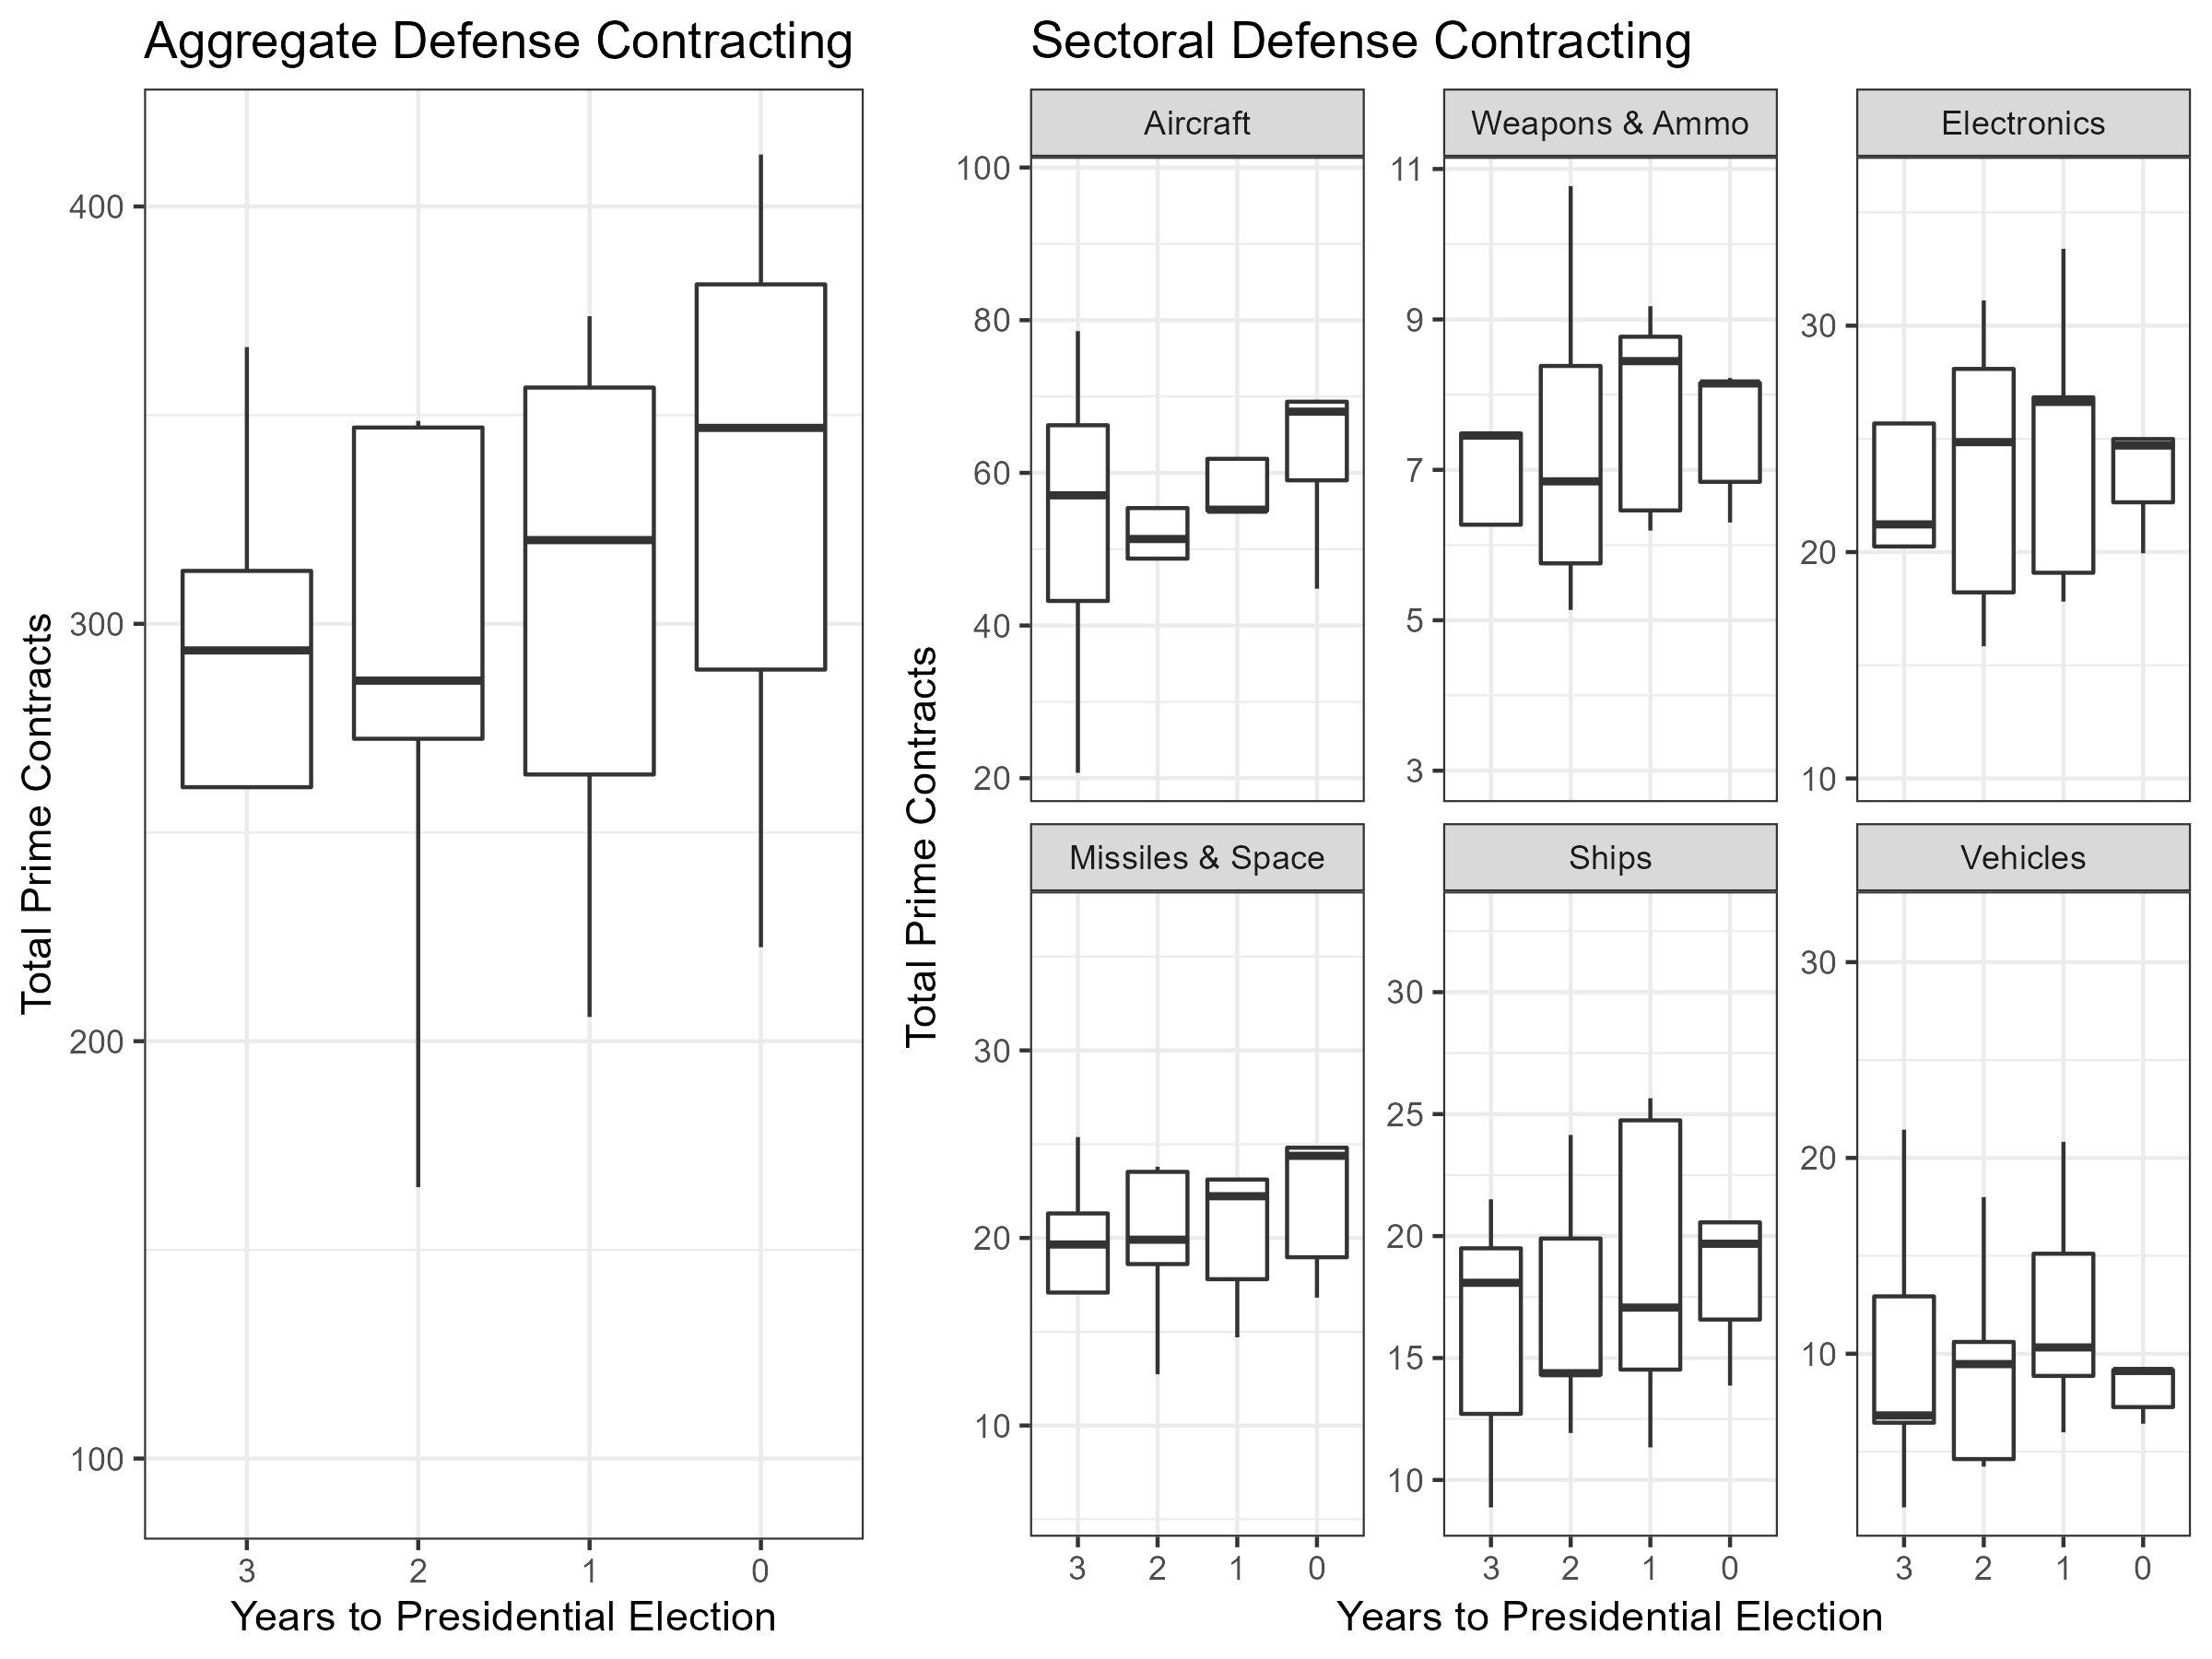
\includegraphics[width=0.95\textwidth]{../figures/contract-cycles.png}
	\caption{Distribution of prime defense contract awards by presidential election proximity, 2000-2020. The dark line in the box plot marks the median value of total contract awards in each year.}
	\label{fig:contract-cycles}
\end{figure}


Particular sectors drive the aggregate increase in defense contracting. 
Aircraft contracts increase dramatically, as do missile and space outlays. 
Naval contacts and prime awards for weapons and ammunition also increase, but retain a high level in the first year of many administrations, which changes those cycles. 
Electronics contracting also rise significantly, and there is a slight increase in vehicle contracting. 
Outside of aircraft, most of the specific platform cycles change the median contract outlay by less than \$10 billion.


Therefore, there is some evidence that defense contracting cycles follow presidential elections.
Along with prior research \citep{DerouenHeo2000}, this suggests that defense contracting is a plausible source of electoral cycles in arms exports from the United States to its allies.
Efforts to manipulate economic conditions through defense contracting have international ramifications. 



\section{Discussion and Conclusion}


All three results are consistent with political budget and defense contracting cycles driving expanding international trade and arms exports to U.S. allies. 
%check for non-linear relationships and adequate support in the interactions \citep{Hainmuelleretal2019}. 
%I also present inferences from Bayesian models that adjust for dyadic clustering through varying intercepts.
Economic efforts to bolster presidential electoral prospects have international consequences. 
Additional goods from defense contracting cycles produce arms flows outside the United States.
This bolsters cooperative relations between the United States and its allies.


Allied economic and security statecraft thus helps U.S. leaders win elections. 
While this is not a part of formal alliance bargains, these informal linkages are essential to grand bargains between alliance patrons and proteges.
Allies need not undertake these cycles deliberately, but their accepting arms transfers is part of a cooperative bundle of ties regardless.


Allied support for political budget cycles affects democratic alliance credibility and maintenance. 
A stable alliance bargain can develop if leaders anticipate the electoral benefits of defense contracting cycles and arms exports to allies.
When leaders expect that maintaining security commitment will have electoral rewards, they will be more likely to invest in alliances. 


These findings also add an international security component to the political budget cycle literature.
Alliance partnerships can allow leaders to manipulate economic conditions for electoral gain. 
By providing an outlet for defense contracting , allies help leaders contract for new goods with less attention to the absorptive capacity and force planning of the U.S. military.


Finally, the argument and findings add to prior findings that states manipulate international economic and security cooperation to bolster or undermine leaders. 
To give one example, \citet{ChyzhUrbatsch2021} show that Chinese soy tariffs reduced support for Republicans in the 2018 midterm elections. 
Allies have both motive and means to use economic and security cooperation to help leaders. 
Rather than undermine leaders, allied arms import decisions create positive inducements for regular cooperation.


Future research could proceed in several directions. 
First, cycles in other economic outcomes such as foreign direct investment, are an interesting area for study. 
Exploring the role of defense industry integration and intermediate goods in these arms cycles is also critical.
Whether these results generalize to autocratic alliances or other democratic alliance patrons is another worthwhile inquiry. 
Security partners of other alliance patrons may take similar actions in different industries, for instance.


In conclusion, political budget cycles reshape international economic and security cooperation.
Budget cycles increase trade and arms transfers to U.S. allies through economic growth and defense contracting.
Security cooperation can therefore facilitate electoral benefits for leaders. 


\newpage
\singlespace
 
\bibliography{../../MasterBibliography} 


\end{document}